\documentclass[a4paper,
fontsize=11pt,
%headings=small,
oneside,
numbers=noperiodatend,
parskip=half-,
bibliography=totoc,
final
]{scrartcl}

\usepackage{synttree}
\usepackage{graphicx}
\setkeys{Gin}{width=.4\textwidth} %default pics size

\graphicspath{{./plots/}}
\usepackage[ngerman]{babel}
\usepackage[T1]{fontenc}
%\usepackage{amsmath}
\usepackage[utf8x]{inputenc}
\usepackage [hyphens]{url}
\usepackage{booktabs} 
\usepackage[left=2.4cm,right=2.4cm,top=2.3cm,bottom=2cm,includeheadfoot]{geometry}
\usepackage{eurosym}
\usepackage{multirow}
\usepackage[ngerman]{varioref}
\setcapindent{1em}
\renewcommand{\labelitemi}{--}
\usepackage{paralist}
\usepackage{pdfpages}
\usepackage{lscape}
\usepackage{float}
\usepackage{acronym}
\usepackage{eurosym}
\usepackage[babel]{csquotes}
\usepackage{longtable,lscape}
\usepackage{mathpazo}
\usepackage[normalem]{ulem} %emphasize weiterhin kursiv
\usepackage[flushmargin,ragged]{footmisc} % left align footnote
\usepackage{ccicons} 

%%%% fancy LIBREAS URL color 
\usepackage{xcolor}
\definecolor{libreas}{RGB}{112,0,0}

\usepackage{listings}

\urlstyle{same}  % don't use monospace font for urls

\usepackage[fleqn]{amsmath}

%adjust fontsize for part

\usepackage{sectsty}
\partfont{\large}

%Das BibTeX-Zeichen mit \BibTeX setzen:
\def\symbol#1{\char #1\relax}
\def\bsl{{\tt\symbol{'134}}}
\def\BibTeX{{\rm B\kern-.05em{\sc i\kern-.025em b}\kern-.08em
    T\kern-.1667em\lower.7ex\hbox{E}\kern-.125emX}}

\usepackage{fancyhdr}
\fancyhf{}
\pagestyle{fancyplain}
\fancyhead[R]{\thepage}

% make sure bookmarks are created eventough sections are not numbered!
% uncommend if sections are numbered (bookmarks created by default)
\makeatletter
\renewcommand\@seccntformat[1]{}
\makeatother


\usepackage{hyperxmp}
\usepackage[colorlinks, linkcolor=black,citecolor=black, urlcolor=libreas,
breaklinks= true,bookmarks=true,bookmarksopen=true]{hyperref}

%meta
%meta

\fancyhead[L]{K. Schuldt \& R. Mumenthaler \\ %author
LIBREAS. Library Ideas, 32 (2017). % journal, issue, volume.
\href{http://nbn-resolving.de/}
{}} % urn 
% recommended use
%\href{http://nbn-resolving.de/}{\color{black}{urn:nbn:de...}}
\fancyhead[R]{\thepage} %page number
\fancyfoot[L] {\ccLogo \ccAttribution\ \href{https://creativecommons.org/licenses/by/3.0/}{\color{black}Creative Commons BY 3.0}}  %licence
\fancyfoot[R] {ISSN: 1860-7950}

\title{\LARGE{Partizipation in Bibliotheken. Ein Experiment, eine Collage}} % title
\author{Karsten Schuldt, Rudolf Mumenthaler} % author

\setcounter{page}{1}

\hypersetup{%
      pdftitle={Partizipation in Bibliotheken. Ein Experiment, eine Collage},
      pdfauthor={Karsten Schuldt, Rudolf Mumenthaler},
      pdfcopyright={CC BY 3.0 Unported},
      pdfsubject={LIBREAS. Library Ideas, 32 (2017).},
      pdfkeywords={Partizipation, Bibliothek, Ausbildung},
      pdflicenseurl={https://creativecommons.org/licenses/by/3.0/},
      pdfcontacturl={http://libreas.eu},
      baseurl={http://libreas.eu},
      pdflang={de},
      pdfmetalang={de}
     }



\date{}
\begin{document}

\maketitle
\thispagestyle{fancyplain} 

%abstracts

%body
\section{1. Vorwort: Irritationen im
Seminar}\label{vorwort-irritationen-im-seminar}

Sommersemester 2017, im Unterricht an der HTW Chur: \enquote{Ich
verstehe immer noch nicht, was genau Sie von mir wollen.} Eine
Studierende hielt mit diesem Satz die ganze Arbeit im Seminar an.

Wir, die beiden Autoren dieses Textes, waren als Professor respektive
Wissenschaftlicher Mitarbeiter für Bibliothekswissenschaft
selbstverständlich auch in der Lehre aktiv. Neben regelmäßig zu gebenden
Kursen, die man inhaltlich updaten kann, aber die doch immer wieder
ähnlich ablaufen, sind Seminare die Königsdisziplin. In ihnen kann man
mit den Studierenden eine offene Fragestellung bearbeiten. Es geht nicht
um konkrete Ergebnisse, sondern darum, zu lernen, selbstständig an
realen Problemen zu forschen und zum Beispiel auch damit umzugehen, wenn
dies keine oder negative Ergebnisse bringt. Es geht ums eigenständige
Forschen. Wir haben mit diesen Seminaren sehr gute, motivierende
Erfahrungen gemacht und die Erkenntnisse (oder Nicht-Erkenntnisse) gerne
auch publiziert. (Haas, Mumenthaler \& Schuldt 2015; Schuldt \&
Mumenthaler 2015)

Aber diesmal war es anders: Das Thema des Seminars lautete
\enquote{Partizipation in Bibliotheken}. Wieder einmal war ein Thema im
Bibliothekswesen als neuer Trend aufgetaucht und wir hatten Zweifel.
Zusammen mit den Studierenden wollten wir untersuchen, (a) was das
überhaupt heisst, (b) was im Bibliothekswesen -- der Schweiz --
überhaupt partizipativ gemacht werden könnte und (c) wie man in
Bibliotheken partizipativ forschen kann. Das ist recht viel, aber wir
wollten die Studierenden entscheiden lassen, partizipativ, in welcher
Richtung sie eigentlich forschen wollten. Der oben angeführte Satz fiel
in der dritten Sitzung, ganz am Ende. Die Sitzungen waren immerhin je
vier Stunden lang. Zuvor waren die Studierenden und wir nicht untätig
gewesen.

In der ersten hatten wir das Feld umrissen -- was ist alles zur
Partizipation zu sagen, welche Zweifel haben wir bei dem Thema (das Wort
\enquote{Pseudopartizipation} kam ständig auf), warum ist das doch ein
Trend,\footnote{Wir konnten auf aktuelle Publikationen aus Deutschland
  (Dewosch 2016; Ilg 2016), den USA (Sharman 2017), Grossbritannien
  (Priestner \& Borg 2016), Dänemark (Rasmussen 2016) und Frankreich
  (Bats 2015) verweisen.} was könnte man für Fragen stellen? Wir hatten
Projekte vorgestellt, die in der aktuellen bibliothekarischen Literatur
\enquote{partizipativ} genannt wurden sowie Methoden der partizipativen
Forschung präsentiert. Zudem führten wir einen (reduzierten) Co-Design
Workshop durch. In der zweiten Sitzung veranstalteten wir mit den
Studierenden dann einen Design Thinking Workshop. Beide Workshop-Formen
gelten in der Literatur als \enquote{partizipativ}, die Studierenden
sollten erfahren, wie es sich als Teilnehmende in diesen anfühlt. Wir
haben -- der eine mehr als der andere -- unsere eigene Kritik an diesen
Formen von Partizipation, aber sie sind das, worüber Bibliotheken heute
reden. Wir diskutierten mit den Studierenden, was die Workshops selber
gebracht hätten.

In der dritten Sitzung nun sollten die Studierenden partizipativ -- das
Thema des Seminars sollte auch das Seminar selber leiten --
untereinander Themen und Forschungs-/Projektmethoden diskutieren und am
Ende ungefähr wissen, was sie (in Gruppen) in der Folge bearbeiten
würden. Wir wollten das alles recht offen lassen. Die Studierenden
entwickelten erst Ideen, schrieben sie nieder, lasen sie gegenseitig und
diskutierten sie. Dann erst entschiedenen sie sich für die, die sie
selber angehen würden. Was für eine gute Idee, dachten wir. Freie
Diskussion, keine Eile beim Thema-Suchen, ein Prozess, wo alle etwas
sagen, sich einbringen können und dazu wenig Druck. Mehrfach hatten wir
betont, dass die Noten für das Umgehen mit den Herausforderungen -- und
eben nicht für ein richtiges / falsches Ergebnis -- erteilt werden.
Zumal wir Noten nicht so wichtig fanden. Wer mitmacht, besteht schon. Es
sollte ums eigene Forschen gehen. Partizipation statt Leistungsdruck.

Und dann das. Andere Gruppen von Studierenden hatten schon ihre Themen
gewählt, aber die Gruppe, der die Studierende angehörte, kam nicht dazu.
Vielmehr machte sie uns klar, dass unsere Vorstellung, Partizipation im
Klassenraum zu ermöglichen, eher zu Unsicherheiten geführt hatte.
\enquote{Ich verstehe immer noch nicht, was genau Sie von mir wollen.}
Wir diskutierten, was wir von den Studierenden wollten: Dass sie sich
selbstständig, im Austausch mit vielen (Partizipation im Sinne einer
gemeinsamen Meinungsbildung) für ein Thema entscheiden sollten, das sie
dann angehen würden. Entweder als Forschung oder als Projekt. Aber
andere Studierende machten uns klar, dass das ja sehr nett von uns
dahergesagt wäre: Freie Wahl, freie Diskussion, Offenheit bei Themenwahl
und Projektergebnissen, ihnen Macht über die eigene Arbeit geben. Aber
am Ende des Seminars waren es immer noch wir beide -- die Autoren dieses
Textes --, die die Macht hatten, Noten zu geben.\footnote{Sicherlich
  könnte man weitergehen und Studierende an der Notengebung beteiligen.
  Auch das wird unter dem Begriff \enquote{Partizipation} diskutiert,
  ist aber zumindest an unserer Hochschule explizit untersagt. Da hat
  jemand anders die Macht, darüber zu bestimmen.}

Was war passiert? Es war so schön ausgedacht: Die Studierenden dürfen in
einem Seminar zur Partizipation im Rahmen partizipativ sein (dass es
einen Rahmen braucht, hatten wir in Seminaren zuvor gelernt; auch dass
es wichtig war, darauf hinzuweisen, dass der Weg und die eigene Arbeit
bewertet werden, nicht das richtige oder falsche Ergebnis). Stattdessen
kam das ganze zu einem Halt. Wir waren irritiert. Alle -- Dozenten und
Studierende.

\section{2. Bibliotheken und Partizipation: Ansprüche, Wünsche, Realität
und
Kontrapunkte}\label{bibliotheken-und-partizipation-anspruxfcche-wuxfcnsche-realituxe4t-und-kontrapunkte}

Das genannte Seminar fand statt, weil wir im Laufe eines
Forschungsprojektes einige Zweifel mit der Verwendung des (politisch
aufgeladenen) Begriffs \enquote{Partizipation} bekamen. In diesem Text
schildern wir unseren Weg zu dem Thema über ein norwegisches
Forschungsprojekt (2.1) und bibliothekarische Literatur (2.2), die wir
in diesem Zusammenhang konsultierten. Anschliessend stellen wir ein
Modell vor, welches unser Unbehagen vielleicht etwas besser greifbar
macht (2.3) und zeigen -- neben zwei notwendigen Exkursen (2.4, 2.6) --,
dass Partizipation in Bibliotheken auch ganz anders verstanden werden
könnte (2.5). Letzteres passt zwar gut in das Modell, welches wir
vorstellen, öffnet aber nur weitere Fragen für die Bibliotheken und die
Bibliotheksforschung, die wir am Ende des Textes präsentieren (3.)

\subsection{2.1 Norwegen}\label{norwegen}

Der Einstieg in das Thema \enquote{Partizipation und Bibliotheken} fand
für die beiden Autoren nicht über die Projekte an deutschen und
schweizerischen Bibliotheken statt, sondern über das Forschungsprojekt
ALMPUB (The ALM-Field, Digitalization, and the Public Sphere\footnote{\href{https://almpub.wordpress.com/}{\emph{https://almpub.wordpress.com/}},
  ALM löst sich auf in \enquote{Archives, Libraries and Museums}, wäre
  also mit dem Begriff \enquote{Gedächtnisinstitutionen} aus der
  deutschsprachigen Diskussion zu übersetzen, obwohl dieser Begriff eine
  Funktion (\enquote{Gedächtnis}) betont, die im Forschungsprojekt wenig
  Bedeutung einnimmt.}), das von Kolleginnen und Kollegen in Norwegen
geleitet wird. Dieses umfasst Forschende aus Norwegen, Schweden,
Dänemark, Deutschland, der Schweiz, Ungarn und den USA. Finanziert wird
es vom Norwegischen Forschungsrat (Noregs forskingsråd).

Die Hauptfrage in diesem Projekt ist, wie Bibliotheken, Archive und
Museen als Einrichtungen in der öffentlichen Sphäre in den heutigen
Gesellschaften, insbesondere bezogen auf die \enquote{Digitalisierung},
agieren. Ein Fokus ist die Produktion von Medien durch Nutzerinnen und
Nutzer (\enquote{\emph{user generated content}}).

Der Projektantrag wurde, da er für den Norwegischen Forschungsrat
verfasst wurde, auch mit Argumenten, die auf die norwegische
Gesellschaft zutreffen, untermauert. Die internationalen Partnerinnen
und Partner sollen praktisch die Forschung, wie sie in Norwegen geplant
und durchgeführt wird, in ihrem jeweiligen Land spiegeln; anschliessend
sollen die unterschiedlichen Perspektiven zusammengebracht werden. Aus
diesem Grund baut der Antrag auch auf den Aufgaben von Bibliotheken (und
Archiven und Museen) auf, wie sie in Norwegen verstanden werden,
insbesondere dem Artikel 100 der norwegischen Verfassung, welcher den
Behörden des Staates die Aufgabe auferlegt, die Voraussetzungen --
sprich die Infrastruktur -- für einen offenen und aufgeklärten (im Sinne
der Aufklärung) Meinungsaustausch in der Gesellschaft zu
schaffen.\footnote{In der offiziellen englischen Übersetzung heisst
  dieser Satz (Artikel 100, letzter Satz): \enquote{The authorities of
  the state shall create conditions that facilitate open and enlightened
  public discourse.}
  (\href{https://www.stortinget.no/globalassets/pdf/english/constitutionenglish.pdf}{\emph{https://www.stortinget.no/globalassets/pdf/english/constitutionenglish.pdf}})}

Im Projektantrag und den Diskussionen in der Forschungsgruppe wurde
sichtbar, dass die Kolleginnen und Kollegen aus Norwegen sowie Schweden
und Dänemark die Aufgabe der Bibliotheken gerade darin sahen, Personen
zu unterstützen, selber digitale Medien zu erstellen -- wobei hierzu
auch Beiträge in Social Media zählen -- und dies als Partizipation
beschreiben: Nicht als Partizipation an den Arbeitsprozessen der
Bibliotheken, sondern die Bibliothek als Infrastruktur für die
Partizipation an der gesellschaftlichen Diskussion. Diese Vorstellung
von der öffentlichen Diskussion als Basis einer demokratischen
Gesellschaft wurde von ihnen auch direkt auf die Theorie des
kommunikativen Handels und der deliberativen Demokratie von Jürgen
Habermas bezogen. Interessant war dabei, dass es für die Kolleginnen und
Kollegen aus skandinavischen Staaten offenbar selbstverständlich
erschien, dieses Verständnis von Gesellschaft und von den Aufgaben der
Bibliotheken zu vertreten. Für die Autoren -- als Forschende aus der
Schweiz -- und den Kollegen aus Potsdam -- als Forschender für
Deutschland -- war dies nicht einsichtig. Grundsätzlich ist im
akademischen Milieu die Position von Habermas bekannt, aber die Idee,
dass sie in der Schweizer Bundesverfassung oder dem Deutschen
Grundgesetz festgeschrieben werden könnte, ist irritierend. Dass
Bibliotheken es als ihre Aufgabe ansehen könnten -- wie man dies
offenbar für Norwegen, Schweden und Dänemark voraussetzen kann -- die
öffentliche und freie Diskussion aktiv zu unterstützen, war für die
Schweiz und Deutschland auch schwer vorstellbar.\footnote{Im Rahmen des
  Projektes konnte dann für die Schweiz auch gezeigt werden, dass diese
  Vorstellung weder in den Gesetzen, Richtlinien, Reglementen et cetera
  über Bibliotheken noch in den Selbstbeschreibungen von Bibliotheken zu
  finden ist.}

Für die Frage, ob und wie Partizipation und Bibliotheken aufeinander
bezogen werden können, ist dies ein wichtiger Hinweis: Diese Beziehung
ist offenbar nicht einfach überall gleich, sondern von Besonderheiten
der jeweiligen Gesellschaften abhängig und wohl auch von den
Besonderheiten des jeweiligen Bibliothekssystems. Man kann nicht einfach
die eigenen Vorstellungen davon, wie Bibliotheken partizipativ agieren
können auf alle Bibliotheken übertragen. Wenn es solche Unterschiede
zwischen eigentlich nicht so unterschiedlichen Gesellschaften gibt, ist
nur zu erwarten, dass es innerhalb der Gesellschaften -- also in der
Schweiz, in Deutschland et cetera -- ebenso grosse Unterschiede geben
wird. Das Forschungsprojekt zeigt aber auch, dass es möglich ist, sich
Bibliothekssysteme vorzustellen, die den expliziten Auftrag haben,
Partizipation zu ermöglichen.

\subsection{2.2 Beispiele aus der bibliothekarische
Literatur}\label{beispiele-aus-der-bibliothekarische-literatur}

\section*{2.2.1 Deutschsprachige
Literatur}\label{deutschsprachige-literatur}

Partizipation, auch in Übersetzungen wie \enquote{Beteiligung}, ist kein
unbekannter Begriff im Bibliothekswesen, sondern scheint in den letzten
Jahren immer wieder in Projekten und Texten Verwendung zu finden.
Auffällig ist, dass diese Arbeiten allerdings das Konzept immer wieder
neu einführen, was nicht nötig wäre, wenn allgemein der Eindruck
vorherrschen würde, dass es etabliert wäre.

Dewosch (2016) liefert in ihrer Bachelorarbeit vor allem eine Sammlung
von Beispielen, die in Bibliotheken durchgeführt wurden. Diese Arbeit
erhebt nicht den Anspruch, einen vollständigen Überblick zu geben,
versucht aber dennoch eine Systematisierung. Grundsätzlich scheint sie
exemplarische Projekte darzustellen, die sich so oder so ähnlich auch in
anderen Bibliotheken in Deutschland (und der Schweiz) finden, wenn man
die bibliothekarische Literatur überblickt. (Unter anderem Grenacher \&
Lienhard 2017; Wildemann 2017; Bergmann \& Flicker 2016; Eigenbrodt
2016; Ilg 2016; Seidl \& Vonhof 2016.)

So erwähnt sie ein Projekt der Stadtbücherei Tübingen,
\enquote{Bürgerbeteiligung organisieren -- Mitreden erwünscht} (Dewosch
2016:21-28), in welchem in verschiedenen -- von Studierenden
durchgeführten -- Teilprojekten die Meinung der Bevölkerung zur weiteren
(möglichen) Entwicklung der Bibliothek eingeholt wurde: Mittels
\enquote{Fokusgruppen},\footnote{Dewosch (2016) schreibt, dass diese
  Gespräche \enquote{in gemütlicher Atmosphäre} (Dewosch 2016:23)
  stattfanden und Teilnehmende \enquote{ihre ideale Bibliothek
  (\ldots{}) beschreiben (konnten)} (Dewosch 2016:23), was wohl eher
  einem Gruppeninterview und nicht einer Fokusgruppe -- bei der die
  Interaktionen der Teilnehmenden, die entstehenden Konsense und
  Differenzen, die innerhalb der Diskussion entstehen, untersucht werden
  und es gerade darum geht, diese Diskussionen anzustossen, nicht
  gemütliche Atmosphäre herzustellen -- entspricht. Deshalb ist es hier
  in Anführungszeichen gesetzt.} in einem Workshop, bei dem mit
Bausteinen von Bürgerinnen und Bürgern Bibliotheken gebaut wurden sowie
drei (öffentlich zugänglichen) Podiumsdiskussionen. An einem Samstag
wurden zudem mehrere Stationen aufgebaut: An einer bastelten Jugendliche
Bibliotheken in Schuhkartons, an einer anderen warfen Bürgerinnen und
Bürger Antworten zu der Fragen, was an der Bibliothek gut und was
geändert werden könnte, in eine Box. An einer dritten konnten Menschen
ihre Ideen zur \enquote{Bibliothek der Zukunft} aufschreiben oder
zeichnen und anschliessend an eine Tafel heften. Die vierte Station
ermöglichte, dass über die allgemeine Ausrichtung der Bibliothek
abgestimmt werden konnte (mit Steinen, die jeweils bei vorgegebenen
Antworten gesammelt wurden) und eine letzte Station, \enquote{Ranking},
liess Menschen an einer Tafel Bilder, welche Angebote der Bibliothek
symbolisierten, in eine Reihenfolge bringen. Die Erfahrungen aus diesen
Projekten benutzte die Bibliothek, um ihre Strategie zu bestimmen.

Aus der Universitätsbibliothek Rostock berichtet Dewosch (2016:28-31)
über eine Online-Umfrage und Co-Design-Workshops, bei denen Studierende
wieder eine ideale Bibliothek am jetzigen Standort zeichneten und
anschliessend in einem Interview befragt wurden. Zudem wurden
Studierende von der Bibliothek auf eine Rundreise zu anderen
Bibliotheken geschickt, um sich die dortigen Lernräume anzuschauen, und
anschliessend ihre Positiv- sowie Negativpunkte zu schildern. Zuletzt
besuchten Studierende einer anderen Hochschule die Bibliothek in Rostock
und beschrieben ihre Eindrücke als potentielle Nutzende. Ergänzt wurde
dies durch einen Gedichtwettbewerb (\enquote{Dichte, was du lernst!}).
Auch hier benutzt die Bibliothek diese Erfahrungen, um die eigene
Strategie zu entwickeln. (Ausführlich auch in Ilg 2016.)

Für die Bücherhallen Hamburg beschreibt Dewosch (2016:32-36) die Arbeit
mit Freiwilligen -- die in Hamburg institutionalisiert ist und unter
anderem einen Beirat aus Freiwilligen umfasst, der sich zu den Projekten
von Freiwilligen äussern kann -- als Partizipation.

Weiter hinten in ihrer Arbeit nennt Dewosch (2016:54-72) noch einige
andere Formen der Partizipation, die in Bibliotheken (hier vor allem in
Dänemark und den USA) genutzt werden. Einige davon finden sich auch in
der deutschsprachigen Literatur: Beschwerdemanagement, Ausstellungen,
die mit Beteiligung von Bürgerinnen und Bürgern erstellt werden,
Co-Design Workshops und Beiräte.

Für die Systematisierung der Beispiele diskutiert Dewosch (2016:51-54)
verschiedene Modelle, um Partizipation zu fassen. Sie selber nutzt dann
ein einfacheres Modell, aber erwähnt auch mit der \enquote{ladder of
citizen participation} von Sherry Arnstein (1969) ein Modell, welches im
Allgemeinen zur Bewertung des Grades von Beteiligung genutzt und in
diesem Text noch weiter unten (2.3) besprochen wird. Doch auch Dewosch
betont, dass die von ihr aufgeführten Beispiele -- die, wie gesagt,
einen guten Rahmen liefern, in denen andere Beispiele aus der
deutschsprachigen bibliothekarischen Literatur integriert werden können
-- verschiedene Grade von Beteiligung ermöglichen. Sie nennt diese Grade
\enquote{Informieren}, \enquote{Beteiligen} und \enquote{Kooperieren},
wobei gerade der letzte Begriff etwas gross gewählt scheint. Zu diesen
zählt sie Beispiele, in denen Nutzerinnen und Nutzer in Workshops oder
als Beirat Hinweise zur Gestaltung von Bibliotheken und deren Angeboten
geben können. Grundsätzlich aber bleibt auch hier die letzte
Entscheidung, was mit den Hinweisen passieren soll, bei der jeweiligen
Bibliothek.

Die Darstellung bei Dewosch (2016) schärft, wenn man sie etwas gegen den
Strich liest, den Blick dafür, was in Bibliotheken an Partizipation
ermöglicht wird und was nicht. Der Eindruck ist, dass Bibliotheken sich
vor allem Hinweise geben lassen für Themen, die sie schon im Vorhinein
bestimmt und strukturiert haben. Das kann sehr einfach sein oder
elaboriert, es kann einzelne Gruppen umfassen oder aber potentiell alle
Nutzerinnen und Nutzer oder gar die gesamte Bevölkerung. Aber letztlich
legen die Bibliotheken fest, worüber abgestimmt, diskutiert oder ein
Workshop durchgeführt wird, dann haben Personen die Möglichkeit, sich
dazu zu äussern und werden zum Teil aktiv dazu aufgefordert. Aber
durchsetzen können sie ihre Meinung nicht. Die Bibliothek informiert
sich und kann Vorschläge und Trends in den Aussagen aufgreifen -- oder
auch nicht.

Das \enquote{Handbuch für die Zusammenarbeit von Bibliothek und Schule}
des Kantons Zürich zählt unter der Rubrik \enquote{Partizipation} zum
Beispiel folgende Punkte auf: \enquote{Mitbestimmung in der
Medienauswahl}, \enquote{Übernahme der Ausleihe während der Pause},
\enquote{Mithilfe beim Ausrüsten der Medien},
\enquote{Bibliotheksführungen,} \enquote{Bücherrallye durch die
Bibliothek}, \enquote{Wandschmuck}, \enquote{Mitarbeit in der
Lesenacht}, \enquote{Beratung für gute Lektüre},
\enquote{Vorleseanlässe}, \enquote{Lesetipps}, \enquote{Bücherrätsel},
\enquote{Gestalten von Ausstellungenn {[}sic!{]}},
\enquote{Informationsblätter gestalten} (Bildungsdirektion Kanton
Zürich, Amt für Jugend und Berufsberatung, Volksschulamt o.J.) Nur ein
Teil dieser Aktivitäten würde bei Dewosch (2016) überhaupt zur
Partizipation gezählt werden, eigentlich nur der erste. Die Idee hinter
diesen Beispielen ist, laut Handbuch, dass die Schülerinnen und Schüler
\enquote{{[}die{]} Gelegenheit {[}erhalten{]}, sich auf eine dem Alter
entsprechende Art an der Gestaltung des Schulalltags zu beteiligen}
(Bildungsdirektion Kanton Zürich, Amt für Jugend und Berufsberatung,
Volksschulamt o.J.) und damit \enquote{Mitverantwortung für die
Schulgemeinschaft zu übernehmen} (Bildungsdirektion Kanton Zürich, Amt
für Jugend und Berufsberatung, Volksschulamt o.J.). Der pädagogische
Impuls ist also leicht zu sehen. Das Beispiel zeigt aber auch, dass
insbesondere dann, wenn nicht die, die partizipieren, sondern jemand
anders darüber bestimmt, wie \enquote{partizipiert} werden soll, auch
die Interessen letzterer (hier: die Erziehungsaufgabe der Schule)
überwiegen. Das sollte stutzig machen: Ist es Partizipation, wenn jemand
vorgibt, was gemacht werden kann und was nicht? Vor allem, wenn das, was
gemacht wird, wenig an dem ändert, was schon da ist?\footnote{Das
  Handbuch enthält auch einen Abschnitt zur \enquote{Elternpartizipation
  in der Bibliothek} (Bildungsdirektion Kanton Zürich, Amt für Jugend
  und Berufsberatung, Volksschulamt o.J.), der noch mehr auf Mitarbeit
  abzielt.} Die gleichen Fragen stellen sich bei einem Text von Nathalie
Franzen (2017), die Bibliotheken im ländlichen Raum beschreibt, welche
durch die aktive Mitarbeit von Ehrenamtlichen, die Veranstaltungen wie
Dorfkonferenzen durchführen oder Infrastruktur wie Lesetreffs aufrecht
erhalten, zu Zentren des Soziallebens für eine alternde Bevölkerung
geworden sind. Das ist selbstverständlich zu begrüssen, aber im Kontext
dieses Textes interessiert die Wortwahl \enquote{Bürgerengagement},
welche die Autorin für den Titel wählt. Diese impliziert einen direkten
Einfluss der Bürgerinnen und Bürger, aber der Artikel thematisiert
nicht, wie gross dieser Einfluss eigentlich ist. Es drängt sich die
Vermutung auf, dass auch bei den bei Franzen (2017) genannten
Beispielen, \enquote{Mitmachen} mit \enquote{Beteiligung} gleichgesetzt
wird.

Zu dieser Form von Gleichsetzung von \enquote{Mitmachen} und
Partizipation passt auch ein Artikel von Frank Sommer (2014). Er
suggeriert, dass die Mitwirkung von Jugendlichen bei Veranstaltungen in
Bibliotheken dazu führen könne, dass diese die Bibliothek eher besuchen.
Hierbei wird die \enquote{Selbstbeteiligung} (Sommer 2014:547) als
Werbung für die Bibliothek verstanden. Nicht der Inhalt -- der bei einem
Verständnis von Partizipation als Politik wichtig wäre -- scheint
relevant, sondern nur, dass die Jugendlichen eine lebendige Bibliothek
kennen lernen.

Fragt man, wer welche Macht hat, liegt sie bei all diesen
Partizipationsprojekten bei der Bibliothek. Einzig Beiräte könnten
anders strukturiert sein, aber auch sie scheinen vor allem zu beraten.
Es scheint nicht darum zu gehen, dass die Bibliotheken
Entscheidungsmacht abgeben oder auch nur einen Konsens mit anderen
Gruppen suchen, sondern dass sie vor allem nach besseren Methoden für
die Befragung der Nutzerinnen und Nutzer und deren Vorstellungen sucht.
Das muss nicht schlecht sein, aber es hinterlässt einiges Erstaunen: Ist
das schon Partizipation? (Die \enquote{Leiter der Partizipation} (2.3)
wird ermöglichen, diesen Eindruck besser einzuordnen.) Bezogen auf die
Differenzierung, die Dewosch (2016) anwendet, scheint es schnell, als
würden noch ein, zwei Kategorien \enquote{oberhalb} der von ihr
aufgezählten fehlen.

In den letzten Jahren ist ein weiterer Aspekt von Nutzerinnen und
Nutzerbeteiligung in Bibliotheken populär geworden: Nutzergenerierte
Inhalte (user generated content) oder Crowdsourcing (Georgy 2015). Wir
-- die Autoren dieses Textes -- haben zu diesem Thema auch zwei
Bachelorarbeiten ausgeschrieben, wobei diese studentischen Arbeiten vor
allem aktuelle Aktivitäten in diesem Bereich beschrieben und wenig zur
Klärung der grundsätzlichen Fragen beitrugen. (Tadic 2017; Tanner 2017)
Aus der Praxis bekannt ist das Crowdsourcing-Projekt des Bildarchivs der
ETH-Bibliothek, bei dem Nutzerinnen und Nutzer zur Erschliessung von
Bildern beitragen (Graf 2016). Ein durchaus erfolgreiches Projekt, das
sich aber in der Tradition der Mitwirkung innerhalb klarer, von der
Bibliothek gesetzten, Grenzen bewegt.

Erstaunlich ist auch, wie schnell im bibliothekarischen Umfeld
Vorarbeiten zum Thema Partizipation wieder vergessen gehen. Während
aktuell eine ganze Reihe von partizipativen Veranstaltungen beschrieben
werden, sind die Arbeiten, die Heike Stadler zwischen 2010 und 2013 zum
Thema vorlegte, scheinbar vollständig aus dem Diskurs verschwunden. Bei
Dewosch (2016) wird sie zum Beispiel gar nicht mehr rezipiert.

Stadler weitete das Thema Partizipation auf Bürgerhaushalte (Stadler
2011a; Stadler 2011c) und weitere politische Prozesse aus (Stadler 2013;
Stadler 2012a; Stadler 2012b; Stadler 2011b), bei denen Bürgerinnen und
Bürger Bibliotheken nicht nur bei Entscheidungen, welche die
Bibliotheken vorbereitet hatten, berieten, sondern Einfluss auf
weiterreichende Bereiche nahmen (bei Stadler \enquote{konzeptionelle
Bereiche} genannt, Stadler 2011c:199). Zudem betrieb sie 2012 bis 2013
ein Weblog zum Thema (Partizipation -- Bibliothek,
\href{https://bibpartizipation.wordpress.com/}{\emph{https://bibpartizipation.wordpress.com/}}),
der sich zu einer Informationsplattform hätte entwickeln können, aber
kaum zur Diskussion genutzt wurde.

Insbesondere bei den Bürgerhaushalten -- bei denen Teile des kommunalen
Budgets zur öffentlichen Diskussion und Abstimmung gestellt werden --
ist der partizipative Impuls leicht ersichtlich. Hier entscheiden die
Bürgerinnen und Bürger mit dem Wunsch, die politischen Entscheidungen
transparent zu machen. Wenn die Bibliothek in diesem Budget auftauchen
will, muss sie sich in die Diskussionsprozesse einbringen. Obwohl
Stadler zu der Einschätzung gelangt, dass dies für Bibliotheken weit
\enquote{mehr Chancen als Risiken} (Stadler 2011c:196) biete, stellte
sie auch fest, dass das Thema in der bibliothekarischen Literatur
\enquote{zurzeit so gut wie gar nicht vorhanden ist} (2011a:90). Dieser
letzten Einschätzung ist auch heute zuzustimmen. Das \enquote{Vergessen}
der Arbeiten von Stadler (die in der BuB und der LIBREAS. Library Ideas,
also nicht an abgelegenen Orten erschienen) ist ein Hinweis darauf, dass
das Bibliothekswesen bestimmte Themen aufgreift und auch fortschreibt
(in diesem Fall: Partizipation vor allem als Beratung der Bibliothek)
aber von anderen (hier: Partizipation als Einfluss auf die Bibliothek)
nichts zu wissen wollen scheint.

\section*{2.2.2 Englisch- und französischsprachige
Literatur}\label{englisch--und-franzuxf6sischsprachige-literatur}

Während die deutschsprachige bibliothekarische Literatur eine bestimmte
gemeinsame Richtung zu haben scheint, wenn es um das Thema Partizipation
geht, gilt das für die englisch- und französischsprachige nicht. In
dieser herrscht eine grössere Diversität im Verständnis von
Partizipation vor. Zudem gehen einige Texte über die Darstellung von
Beispielen, welche die deutschsprachige Literatur prägen, hinaus.

Während eigentlich zu erwarten ist, dass aufgrund der Häufigkeit des
Themas in bibliothekarischen Zeitschriften ein \enquote{Praxishandbuch
Partizipation in Bibliotheken} in der einschlägigen Reihe des De
Gruyter/Saur-Verlages mindestens in Vorbereitung sein müsste, ohne dass
es dafür Hinweise gibt, liegt ein solches für französische Bibliotheken
mit dem Sammelwerk von Raphaëlle Bats -- die sich auch später noch zu
diesem Thema äusserte -- von 2015 (Bats 2015) schon vor. Sie stellt
Partizipation unter das Thema \enquote{Demokratisierung} (Bats 2016).
Bibliotheken hätten die Aufgabe, demokratische Einrichtungen zu werden
und könnten dies nur, wenn sie die Bevölkerung mit einbeziehen
würden.\footnote{\enquote{Pour ces bibliothèques qui integrent une
  approche participative, celle-ci accompagne leur insertion dans leur
  territoire et l'affirmation de leur nécessaire rôle social et
  politique.} (Bats 2015:9)} Der Anspruch ist weit höher als alles, was
aktuell in der deutschsprachigen Literatur dargestellt wird.\footnote{Eine
  Ausnahme stellt die Masterarbeit von Gerhard Zschau und Peter Jobmann
  (Zschau \& Jobmann 2013) dar, die unter anderem Machthierarchien
  zwischen Bibliothekspersonal und Nutzerinnen / Nutzern thematisiert
  und die Aufgabe von Bibliotheken an der Medienpädagogik orientiert.
  Symptomatisch -- insbesondere in Bezug auf die Erfahrung mit den
  Arbeiten von Heike Stadler -- scheint aber, dass diese Arbeit, und
  damit auch der in ihr präsentierte Ansatz, in der restlichen
  bibliothekarischen Literatur offenbar nicht rezipiert wird. Ebenso
  werden andere bibliothekarische Texte, die zumindest am Rande
  Partizipation behandeln, in der aktuellen Literatur nicht rezipiert,
  zum Beispiel Kaiser (2014). Hier stellt sich die weiterführende Frage,
  die in diesem Text nicht weiter thematisiert werden kann, welche Texte
  im Bibliothekswesen wahrgenommen und welche nicht wahrgenommen werden
  und warum.} Hinzu kommt, dass Bats davon ausgeht, dass der Trend zur
Partizipation in Frankreich ein allgemeiner sei, der nun in Bibliotheken
ankommen würde.\footnote{\enquote{L'accroissement de la participation
  dans la société française au cours de 4, 5 dernières années est
  aujourd'hui bien visible dans les bibliothèques.} (Bats 2015:9)} Das
Buch beginnt mit diesem Anspruch, Bats geht in einem weiteren Text auch
darauf ein, dass die Fähigkeit, sich aktiv partizipativ zu engagieren,
erlernt werden muss.\footnote{Keine originär bei Bats vertretende, aber
  offenbar immer wieder neu formulierte Erkenntnis, siehe das Nachwort
  dieses Textes.} Hieraus würde sich ergeben, dass Partizipation nicht
in einem Projekt alleine durchgeführt werden kann, sondern sich
eigentlich nur mit der Zeit, wenn es zum Normalfall geworden ist,
partizipativ zu arbeiten, die Potentiale von Partizipation einstellen
würden, weil dann die Menschen auch wüssten, was möglich ist.
Anschliessend präsentiert das Buch vor allem Beispiele für Partizipation
in Bibliotheken und Museen. Diese gehen teilweise über die Beispiele,
die Dewosch (2016) zusammengetragen hat, hinaus, indem sie sich Gedanken
darüber machen, was die Grenzen der Partizipation sind oder aber den
Nutzerinnen und Nutzern Infrastruktur (zum Beispiel BiblioBoxen) zur
eigenen Verwendung zur Verfügung stellen. Der Grossteil aber macht das,
was auch aus der deutschsprachigen Literatur bekannt ist: Bei schon
vorgegebenen Grenzen wird die Bevölkerung eingeladen, teilweise in
ausdifferenzierten Verfahren, ihre Meinung abzugeben oder Vorschläge zu
machen.

In der englischsprachigen Literatur findet sich (wieder einmal, wie bei
anderen Themen auch) sehr viel mehr zum Thema selber, aber dies oft in
keinem weiteren Rahmen als in der deutschsprachigen. Insbesondere beim
Einrichten und Umgestalten von Bibliotheken, werden entweder spezifische
Gruppen oder aber \enquote{alle} aufgefordert, in teilweise klar
strukturierter Weise ihre Meinung zu äussern.

Für die USA gibt es, wie für Frankreich, ein Dokument, das man --
zumindest für einen Bereich -- als Handbuch für Partizipation in
Bibliotheken beschreiben könnte: Participatory Design in Academic
Libraries von Nancy Fried Foster (2014). Der Fokus dieses Werks liegt
auf der Beteiligung bei der Umgestaltung von Bibliotheken, aber diesen
Fokus gibt es ja auch in der deutschsprachigen Literatur. Das im Auftrag
des Council on Library and Information Resources erstellte Dokument
präsentiert verschiedene Methoden, diese Beteiligung zu erreichen, immer
mit Beispielen, in denen diese erfolgreich\footnote{Wenn man
  \enquote{erfolgreich} übersetzt mit: Es gab Ergebnisse.} eingesetzt
wurden.\footnote{Nebenbemerkung: Dieses Dokument ist eines, welches
  eigentlich viel Arbeit, die im Bibliotheksbereich lokal gemacht wird,
  ersparen könnte. Immer wieder entwerfen Bibliotheken Projekte, bei
  denen sie für sie neue Methoden ausprobieren und dies später als
  innovativ beschreiben (siehe Ilg 2016), obwohl diese schon ausführlich
  in diesem Dokument beschrieben sind, inklusive dem Nachweis, dass sie
  in Bibliotheken funktionieren. Bibliotheken könnten sich vielmehr auf
  die Durchführung ihrer Projekte konzentrieren, wenn sie auf diesem
  publizierten Wissen aufbauen würden.} Wieder sind alle beschriebenen
Projekte darauf reduziert, dass die Bibliothek vorgibt, worüber
überhaupt mitbestimmt werden darf (und das ist oft nicht viel) und auch
keine Verpflichtung eingeht, umzusetzen, was vorgeschlagen wird. Oft
geht es bei den Methoden darum, bei der Planung den Blick der
Nutzerinnen und Nutzer einzunehmen oder aber diese Vorstellungen (oft
individuell) visualisieren zu lassen.

Eine Anzahl von Texten beschäftigt sich auf einer abstrakteren Ebene mit
Partizipation. Browndorf (2014) befragt zum Beispiel die Einbindung von
Studierenden in die Bibliothek auf die Ziele dieser Einbindung hin.
Leitend ist bei ihr die Frage, wer eigentlich \enquote{spricht}, also
die Möglichkeit hat, sich so zu äussern, dass es einen Unterschied
macht. Zu enge Formen von Partizipation schränken diese \enquote{Macht
zu sprechen} stark ein. Dabei, so ihre Argumentation (die an Bats (2015)
erinnert) müsste eine partizipative Kultur das Gefühl von
\enquote{ownership}\footnote{Also das Gefühl, dass die Bibliothek
  benutzt und verändert werden kann, was mit mehr Verantwortung
  verbunden ist als wenn man einfach Nutzerin oder Nutzer wäre.}
produzieren, auch damit Studierende (um die es ihr geht) nach der
Ausbildung in die Lage versetzt werden, \enquote{ownership} über andere
commons (die Gesellschaft) zu erlangen.

Sung und Hepworth (2013) fragen anhand von drei Case Studies aus
England, ob Bibliotheken eine Rolle beim Erzeugen von Communities
spielen, was bei ihnen als Ermöglichung von Partizipation übersetzt
wird. Sie gehen also von der Frage, ob Bibliotheken mit Beteiligung
besser beraten werden können, zu der Frage über, ob sie Partizipation in
der gesamten Gesellschaft ermöglichen würden. Neben der Erkenntnis, dass
es nur wenig Untersuchungen dazu gäbe, stellen sie grundsätzlich fest,
dass die Öffentliche Bibliothek eine Infrastruktur für diese Form von
Partizipation darstellen kann, aber nur dann sinnvoll genutzt wird, wenn
deren Nutzung als solche verstärkt beworben und motiviert wird.
Ansonsten verbleibt es bei der reinen Möglichkeit, die nicht genutzt
wird. Während sie selber über die Bibliothek hinaus auf die Gesellschaft
schauen, verweisen sie auch darauf, dass unter dem Begriff
\enquote{Community Engagement} (und damit auch dem Verständnis von
\enquote{Beteiligung}) verschiedenes verstanden wurde und insbesondere
von Bibliothekarinnen und Bibliothekaren eher auf die Bibliothek und
nicht die Gesellschaft bezogen wurde. (Siehe auch Huzar 2013)

Dass es sehr unterschiedliche Verständnisse von \enquote{Partizipation}
gibt, zeigt -- für den Archivbereich, aber auch für den
Bibliotheksbereich übertragbar -- Huvila (2015). In einer Diskursanalyse
identifiziert sie fünf unterschiedliche, zum Teil antagonistische
Diskurse: \enquote{Participatory context}, \enquote{Archivists as
participants}, \enquote{Participation as new \enquote{use}},
\enquote{Others as informants}, \enquote{Others-oriented participation}.
(Huvila 2015:373) Solche Darstellungen machen es verständlicher, warum
es so einfach und doch so schwer ist, über Partizipation zu reden: Es
ist oft nicht klar, was gemeint wird.

Bernier, Males \& Rickman (2014) entwerfen zum Beispiel, auf der Basis
einer Umfrage zur Praxis der Planung von Neuausstattung und Bau von
neuen Bibliotheken, einen Youth Participation Index, der hoch ausfällt,
wenn Jugendliche bei diesen Planungen mitreden dürfen. Sie stellen einen
Zusammenhang zwischen hohem Indexwert und höherer Zufriedenheit der
Jugendlichen mit den bibliothekarischen Angeboten, der Nutzung der
Bibliothek sowie einem höheren Interesse der Jugendlichen an ökologisch
nachhaltigen Baumaterialien her. Insoweit hat die Partizipation offenbar
einen positiven Effekt, gleichzeitig können sie auch zeigen, dass es
sich nicht um Ausnahmeprojekte handelt, sondern relativ viele
Bibliotheken in den USA ihre jugendlichen Nutzerinnen und Nutzer
einbeziehen. Nicht alle tun es, aber es ist auch keine
Innovation.\footnote{Dies gilt offenbar auch für die Schweiz, siehe die
  Ergebnisse des Seminars, die im Nachwort dieses Textes referiert
  werden.} Allerdings: Auch hier wieder vor allem im von der Bibliothek
vorgegebenen Rahmen und gemessen an den Interessen der Bibliotheken. Der
potentielle demokratisierende Effekt, den Bats (2015) anspricht,
interessiert Bernier, Males \& Rickman (2014) nicht.

Lankes, Stephens \& Arjona (2015) beschreiben, wie ein spezifisches
Verständnis von Partizipation in die Curricula bibliothekarischer und
musealer (US-amerikanischer) Ausbildungseinrichtungen integriert werden
soll. Auch dieses ist sehr davon geprägt, Partizipation als (bessere)
Form zu finden, um die Interessen der Nutzerinnen und Nutzer zu erheben
und in die bibliothekarische Arbeit zu integrieren: \enquote{In a
participatory culture, information and museums professions must find
ways to shape their goals and services to respond to the needs of the
communities, not the other way around.} (Lankes, Stephens \& Arjona
2015:65) Es geht ihnen -- auch über diesen einen Text hinaus, wie Lankes
(2011; 2012) zeigt -- schon darum, dass Bibliotheken offener werden, auf
die Gesellschaft zugehen und auf diese hören. Aber auch hier mit dem
Vorbehalt, dass am Ende die Bibliothek entscheidet und diese
Entscheidungen dann als positiv für die Gesellschaft präsentiert (Lankes
2012).

Daneben gibt es aber auch relativ viele Beiträge, die von partizipativen
Projekten berichten wollen, bei denen sich schnell die Frage stellt, ob
das wirklich Partizipation ist. Hattwig, Lam \& Freidberg (2015) stellen
beispielsweise ein Projekt vor, bei dem Studierende im Rahmen ihres
Studiums eine digitale Sammlung zu einem lokal-historischen Thema
anlegten, dazu auch Videos (oral history) aufnahmen, und diese,
inklusive Metadaten, in ein Repository einstellten. Partizipativ daran
sei, dass die Studierenden diese Arbeit selber gemacht hätten, nach
einem Plan, der zuvor von Unterrichtenden und Bibliothek ausgearbeitet
worden war. Veláquez (2016) beschreibt einen Teen Space, der relativ
flexibel ist und bei dem Jugendlichen gestattet wird, ihn umzunutzen --
zum Beispiel ihn weniger \enquote{nett} machen, damit Erwachsene nicht
kommen und der Raum eher für die Jugendlichen allein funktioniert -- als
partizipativ.\footnote{Aber auch hier mit dem Hintergedanken, dass es
  der Bibliothek hilft: \enquote{Participatory space helps facilitate
  library-based programming for teens while keeping these activities in
  close proximity to the teen book collection, thereby increasing
  connections to reading and literacy.} (Veláquez 2016:32)}

Auf der Basis eines Toolkits der ALA, in dem Ansätze von
partizipatorischen Projekten gesammelt werden,\footnote{Jetzt als
  \enquote{Libraries Transforming Communities} unter
  \href{http://www.ala.org/tools/librariestransform/libraries-transforming-communities}{\emph{http://www.ala.org/tools/librariestransform/libraries-transforming-communities}}.
  {[}25.08.2017{]}} beschreibt Stewart (2015), wie er in einer
Schulbibliothek verschiedene Mitglieder der Schulgemeinschaft in Gruppen
an der Gestaltung der Bibliothek mitwirken liess, was vor allem über
empathisches Zuhören geschah. Grösser, aber mit ähnlicher Aussage
beschreibt Désilets (2017) für die Öffentlichen Bibliotheken in
Montreal, dass diese vor allem durch den Versuch, die
(unterschiedlichen) Interessen der Nutzerinnen und Nutzer wahrzunehmen
und diesen entsprechend Angebote zu planen, partizipativ seien. Während
dies allerdings bei Stewart in einer Schule noch nachvollziehbar wirkt
-- er beschreibt sogar, wie er nach einer Weiterbildung mit dem
empathischen Zuhören begann --, lässt sich bei den Beschreibungen von
Désilets schon kaum noch erkennen, was daran normale bibliothekarische
Entwicklung und was daran partizipativ sein soll.

\subsection{2.3 Leiter der Partizipation (Arnstein
1969)}\label{leiter-der-partizipation-arnstein-1969}

Ein Modell, welches bei der Diskussion von Partizipation in ganz
verschiedenen Kontexten immer wieder auftaucht, ist die schon erwähnte
\enquote{Leiter der Partizipation}. Diese scheint auch deshalb so oft
angeführt zu werden, weil es ein Gefühl beschreibbar macht: Dass das
meiste, was als Partizipation bezeichnet wird, eigentlich keine
Partizipation ist, sondern nur eine Übung in Partizipation, weil die
eigentlichen Strukturen, in denen Entscheidungen getroffen werden, nicht
wirklich beeinflusst werden.\footnote{Eventuell ist dieses Gefühl bei
  einem der Autoren (Schuldt) auch biographisch geprägt, da er in der
  DDR noch genügend Aktivitäten kennengelernt hat, die sich demokratisch
  und partizipativ gaben, aber es offensichtlich nicht waren (nur als
  Verweis: Die \enquote{Dialogkampagne} der SED 1989) und danach
  Freiheit kennenlernte (Stichwort: Partizipation als Lernprozess), die
  er später, in der Schweiz zum Teil wieder vermisste (Stichwort:
  Offener Dialog ohne jede Wirkung). Aber die biographische Sicht
  alleine kann nie alles beschreiben.} Es gibt verschiedene
Bezeichnungen dafür: Schein-Partizipation, Teilbeteiligung,
\enquote{trivializing participation} (Roig 2016) und auch verschiedene
Probleme, die man damit haben kann: Die Vermutung, dass nur so getan
werden soll, als gäbe es Beteiligungsmöglichkeiten, vielleicht, um
Entscheidungen, die auch so getroffen werden, als demokratisch
legitimieren zu können; die Angst, dass der demokratische Kern von
Partizipation verloren geht, wenn einfach jede Befragung
\enquote{partizipativ} genannt wird; die Vermutung, dass sich gar nicht
klar gemacht wird, welches Potential für eine demokratischere (bessere)
Gesellschaft in Partizipation steckt; die Vermutung, dass Einrichtungen
nur partizipativ sind, weil es gerade innovativ klingt und dies morgen
wieder vergessen haben werden, weil sie einem anderen Trend nachschauen.
Und gleichzeitig die Einsicht, dass vielleicht nicht alle Einrichtungen
partizipativ sein können oder wollen.

Die \enquote{Leiter} wurde von Sherry R. Arnstein (1969) entwickelt, um
zu untersuchen, wie sehr Projekte der \enquote{citizen participation},
gerade in der Stadtplanung, tatsächliche Beteiligung ermöglichen oder
eher Veranstaltungen ohne Einfluss darstellen. Dies griff Kritik und
Debatten zu Projekten der Stadtplanung in den 1960er Jahren (in den USA)
auf, die aber auch heute (und auch im deutschsprachigen Kontext)
grundsätzlich nicht geklärt sind beziehungsweise immer wieder
auftauchen, wenn über Partizipation und deren Umsetzung diskutiert wird.

Während die bibliothekarische Literatur Partizipation vor allem so zu
verstehen scheint, als ob man sie einfach in der bibliothekarischen
Arbeit nutzen könne oder auch nicht -- also in gewisser Weise als
unpolitisch --, verortet Arnstein Partizipation in politische
Auseinandersetzungen über die Frage, wer die Macht hat, etwas zu ändern
oder aber gehört zu werden.

\begin{quote}
\enquote{The idea of citizen participation is a little like eating
spinach: no one is against it in principle because it is good for you.
Participation of the governed in their government is, in theory, the
cornerstone of democracy -- a revered idea that is vigorously applauded
by virtually everyone. The applause is reduced to polite handclaps,
however, when this principle is advocated by the have-not blacks,
Mexican-Americans, Puerto Ricans, Indians, Eskimos, and whites. And when
the have-nots define participation as redistribution of power, the
American consensus on the fundamental principle explodes into many
shades of outright racial, ethnic, ideological, and political
opposition.} (Arnstein 1969:216)
\end{quote}

Obwohl der spezifisch temporäre US-amerikanische Hintergrund (der ja
Konflikte anspricht, die immer noch nicht gelöst wurden) den Text von
Arnstein prägt, ist, wie schon gesagt, der Ansatz, den sie präsentiert,
um Partizipation zu verstehen, auch in anderen Kontexten genutzt worden.
Sie drückt das allgemeine Gefühl aus, dass vieles, was
\enquote{Partizipation} genannt wird, eigentlich keine ist, weil am Ende
nicht die von der Partizipation profitieren, die sich äussern
\enquote{dürfen}, sondern andere, nämlich vor allem die, die eh schon
die Macht haben, Entscheidungen zu treffen oder sich hörbar zu machen.
Gleichzeitig verbleibt sie nicht bei dieser Vermutung, dass alle
Partizipation nur vorgespielt sei.

Was sie vorschlägt, ist, die unterschiedlichen Formen von Partizipation
zu systematisieren. Dies tut sie in der schon erwähnten \enquote{Leiter
der Partizipation}. Diese \enquote{Leiter} umfasst acht Stufen, die
zudem in drei Ebenen unterteilt sind:

\begin{enumerate}
\def\labelenumi{\arabic{enumi}.}
\item
  Ebene Nicht-Partizipation: Manipulation, Therapie
\item
  Ebene Grade von Tokenism (Alibi-Politik): Information, Anhörung,
  Beschwichtigung
\item
  Ebene Grade der Macht der Bürgerinnen und Bürger: Partnerschaft,
  delegierte Macht, Kontrolle durch Bürgerinnen und Bürger
\end{enumerate}

\begin{figure}
\centering
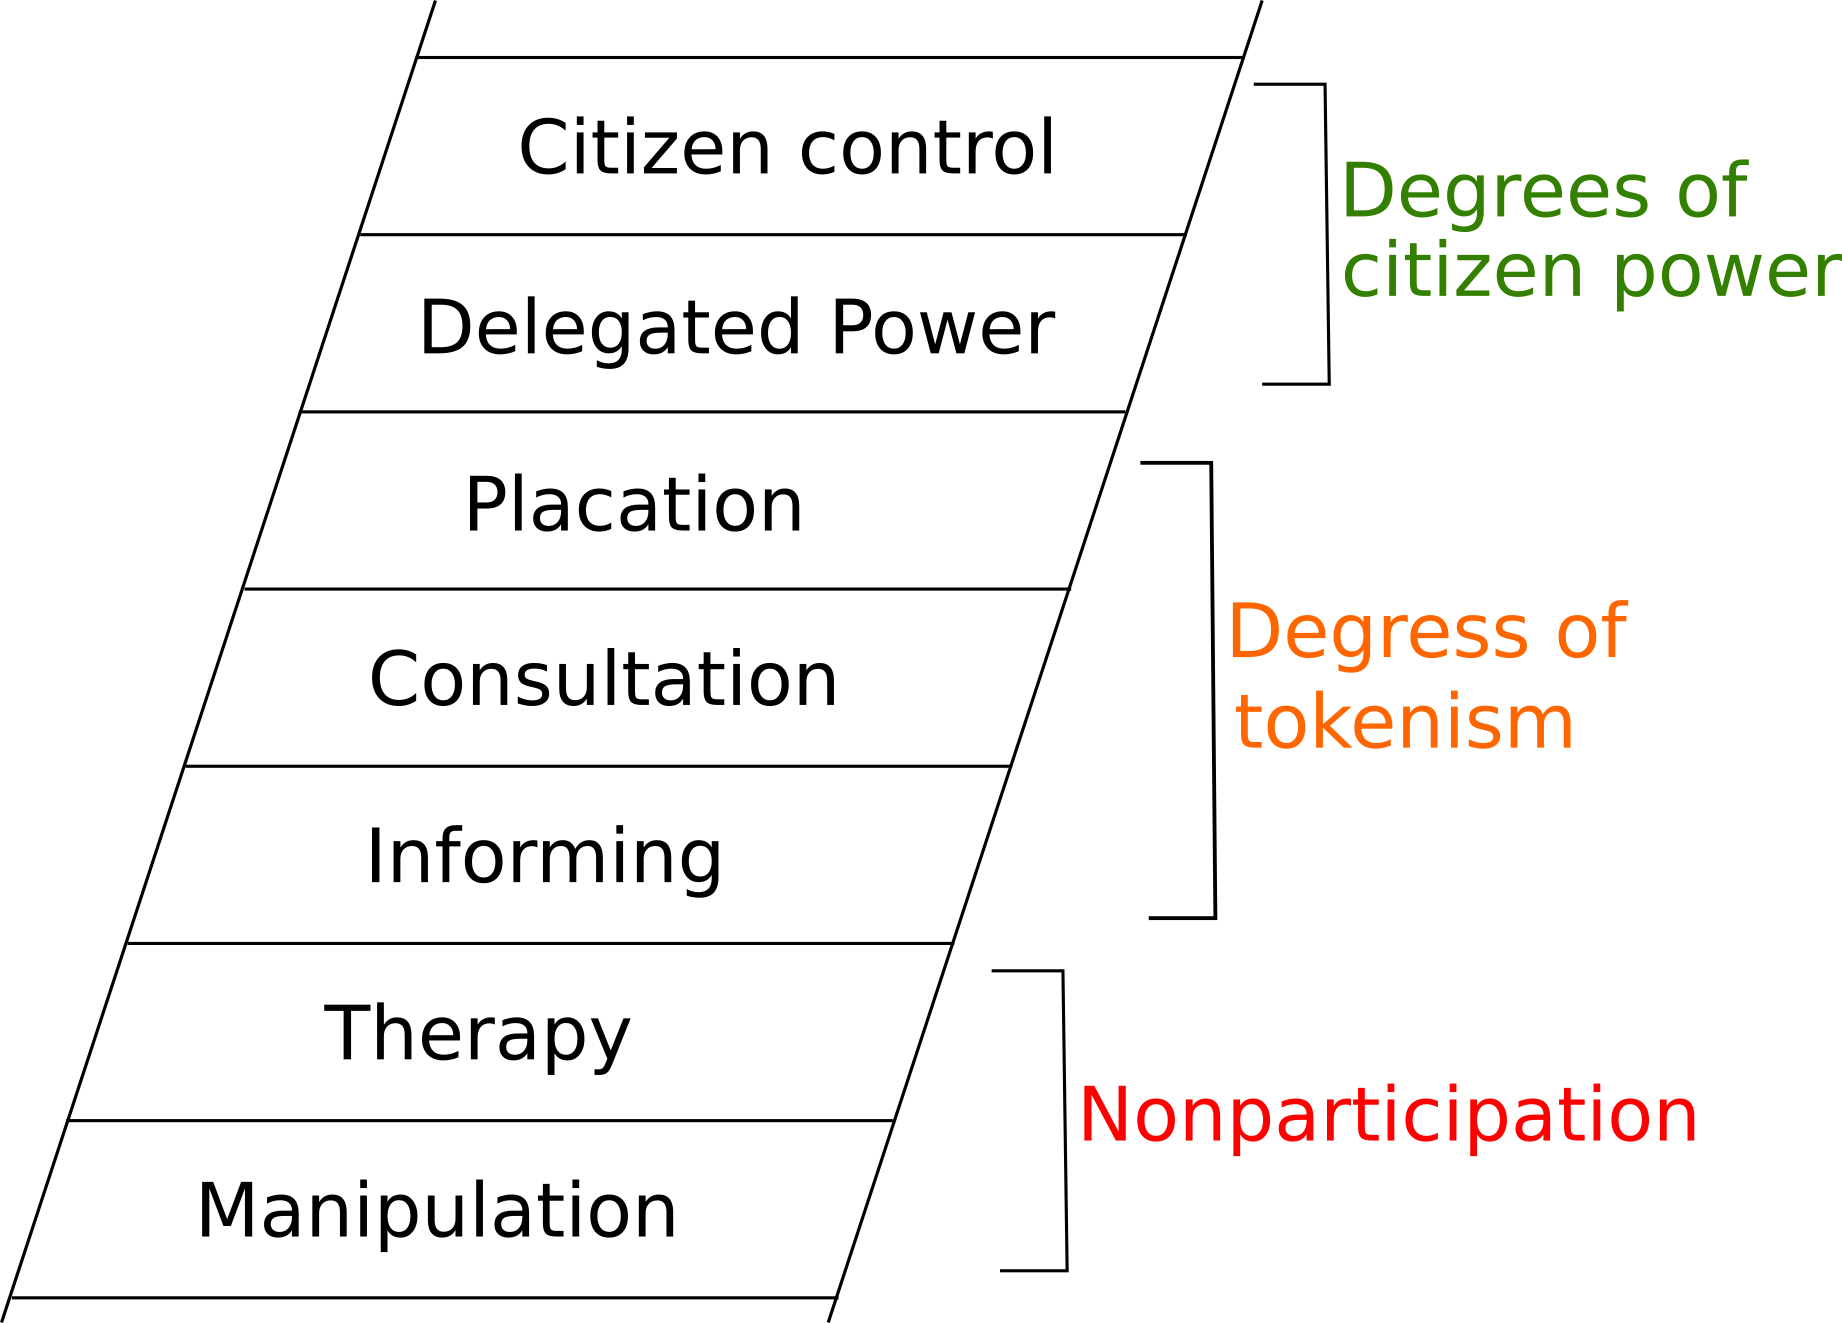
\includegraphics{img/Ladder-of-Citizen-Participation.jpg}
\caption{Leiter der Partizipation (eigene Darstellung nach Arnstein
1969:217)}
\end{figure}

Die Übersetzung der Begriffe ist unterschiedlich, wie gesagt, wurde die
Leiter auch schon mehrfach \enquote{erweitert} oder angepasst (zum
Beispiel in Carpentier 2016). Aber die Grundidee ist gleichbleibend.

\begin{enumerate}
\def\labelenumi{\arabic{enumi}.}
\item
  Das, was \enquote{Partizipation} genannt wird, ist unterschiedlich in
  der Intensität und Möglichkeit der Partizipierenden, Einfluss zu
  nehmen.
\item
  Es gibt Formen von \enquote{Partizipation}, die tatsächlich als
  Pseudo-Partizipation beschrieben werden können. (Arnstein nennt hier
  \enquote{rubberstamp advisory committees} (Arnstein 1969:218), also
  Komitees, Sounding Boards, Beiräte, die eigentlich nur dazu da sind,
  um schon getroffene Entscheidungen abzusegnen.)
\item
  Das Ideal bei Partizipation ist -- wenn man es als Teil demokratischer
  Entscheidungsfindung ernstnimmt --, dass die Betroffenen direkt
  Einfluss nehmen können und zwar grundsätzlich (um im Thema von
  Arnstein zu bleiben, auch die Möglichkeit, bei einer Planung eine ganz
  andere Bebauung durchzusetzen, zum Beispiel mehr Wohnungen statt
  Geschäfte, und nicht nur die Farbe der Gebäude oder die konkreten
  Geräte auf dem Spielplatz mitzubestimmen). Das heisst nicht, dass alle
  alles machen, aber dass alle die Möglichkeit haben, mitzubestimmen.
\item
  Zwischen diesen beiden Polen gibt es einen Bereich von anderen Formen,
  die nicht als reiner \enquote{rubberstamp} aber auch nicht als
  \enquote{volle Partizipation} verstanden werden können. Sollte man sie
  Partizipation nennen? Das ist wohl umstritten. Aber es macht die
  Verunsicherung deutlich, die auftritt, wenn in der bibliothekarischen
  Literatur von Partizipation gesprochen wird, aber es sich doch eher um
  Beratung/Information der Bibliotheken geht.
\item
  Zumeist geht es bei den Projekten im bibliothekarischen Bereich ja
  nicht um Partizipation als Form der demokratischen Kontrolle -- oder
  das \enquote{Lernen von Demokratie} --, sondern darum eine
  Entscheidung über die Ausstattung des Raums, die Strategie der
  Bibliothek oder ähnliches besser zu treffen, als nur durch die
  Bibliothek selber. Deshalb ist es vielleicht auch schwierig zu sehen,
  wie die Bibliothek \enquote{partizipativ} sein könnte, ohne dass den
  bibliothekarischen Projekten vorgeworfen werden müsste, manipulativ
  sein zu wollen. Es herrscht wohl schon ein Interesse daran vor zu
  wissen, was die Nutzerinnen und Nutzer denken; aber nur soweit es
  bestimmte Entscheidungen nicht einfach ändert. Diese Projekte sind
  wohl fast immer in der Ebene \enquote{Tokenism} einzuordnen. Dadurch
  bleibt aber immer der Nachgeschmack, dass es mehr sein könnte, um
  \enquote{wirklich partizipativ} zu sein. Immer.
\end{enumerate}

Nutzt man die Leiter der Partizipation, um die Beispiele, die in diesem
Text angeführt wurden (oder weiter unten noch werden), abzutragen,
scheint die Differenz zwischen den möglichen Ansprüchen an Partizipation
und den tatsächlichen Beispielen verständlicher zu werden. Der Eintrag
von Toronto (vergleiche 2.5.1) deutet aber auch darauf hin, dass es
denkbar ist, über diese Formen der \enquote{einfachen Partizipation}
hinauszugehen.

\begin{figure}
\centering
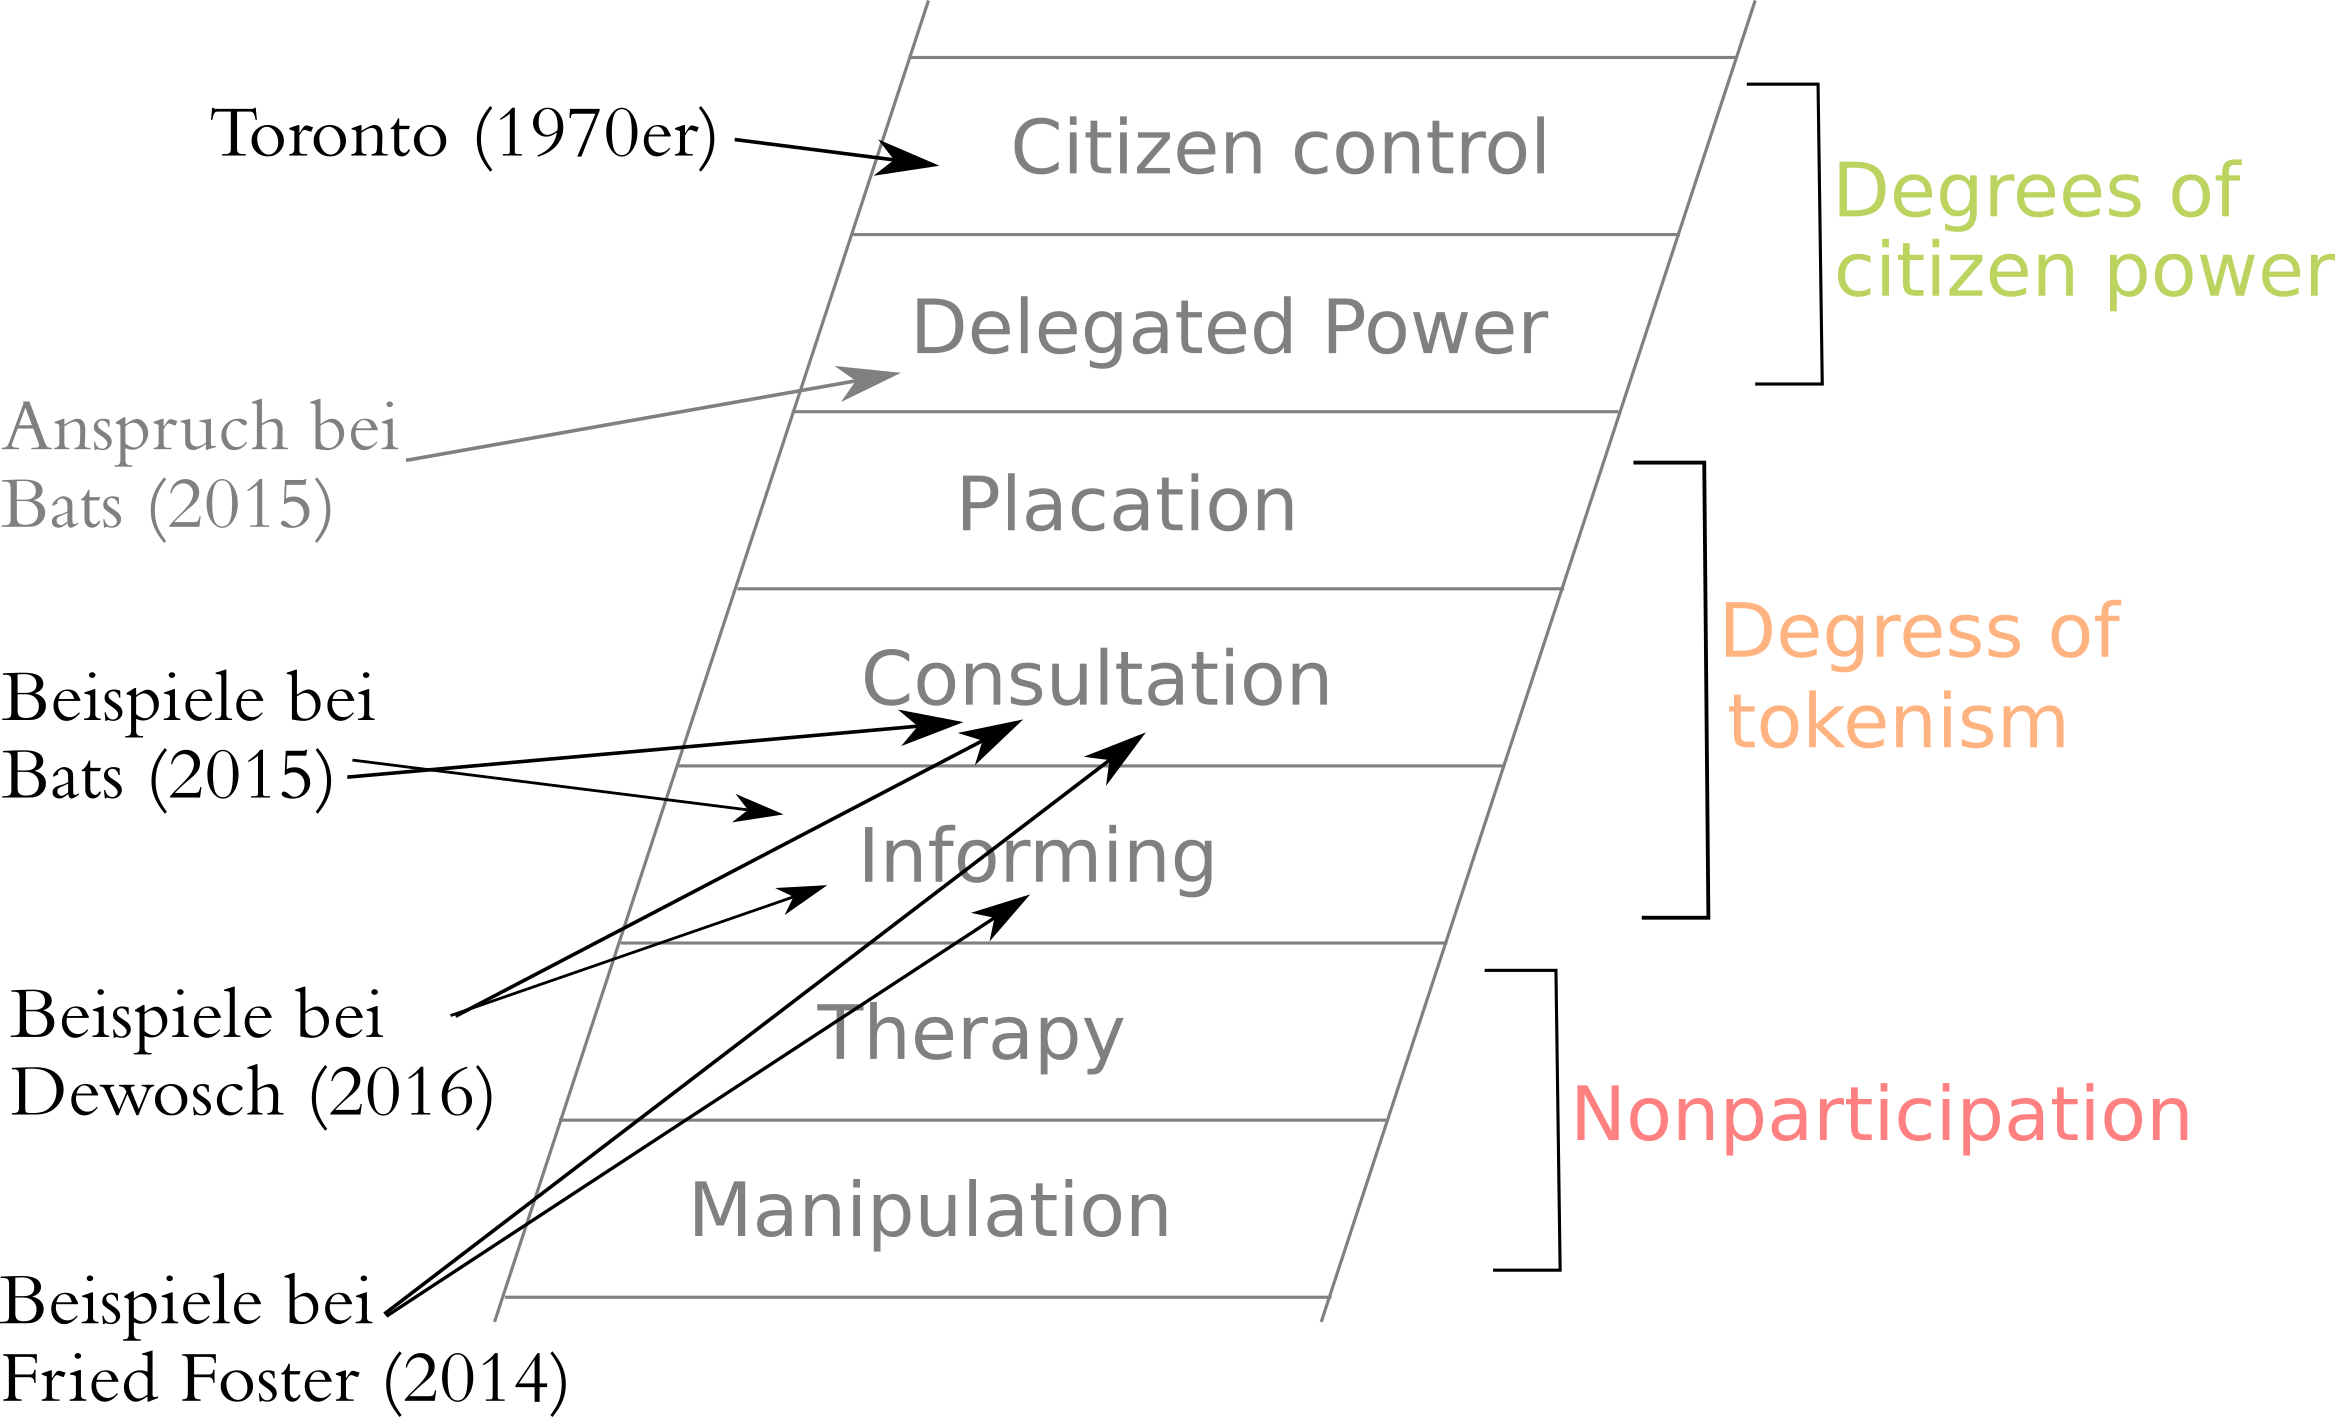
\includegraphics{img/Ladder-of-Citizen-Participation-mitEintraegen.jpg}
\caption{Leiter der Partizipation, mit Einträgen von in diesem Text
angesprochenen Beispielen aus Bibliotheken (eigene Darstellung)}
\end{figure}

\subsection{2.4 Exkurs: Habermas}\label{exkurs-habermas}

Die Leiter der Partizipation von Arnstein mag als einfaches Modell
gelten, welche die Komplexität des Themas fassbarer macht. Aber es gibt
mit Jürgen Habermas einen weiteren Namen, der im Bezug auf das Thema
\enquote{Partizipation} immer wieder genannt wird, nur in den
deutschsprachigen bibliothekarischen Texten nicht. Wie schon
thematisiert (2.1) basiert zum Beispiel die Vorstellung von
Partizipation, die hinter dem Artikel 100 der norwegischen Verfassung
steht, auf den Arbeiten von Jürgen Habermas, dessen Name immer wieder
fällt, wenn es um Fragen des Gelingens von politischen und
gesellschaftlichen Prozessen der modernen Gesellschaft geht. Diese
machen das ganze Feld wieder unübersichtlicher.

Die Arbeiten von Habermas beschäftigen sich unter anderem mit der Frage,
wie die moderne bürgerliche Gesellschaft und damit auch die heutigen
Formen von Demokratie entstanden sind und funktionieren. (Habermas 2004
{[}1962{]}; 1981; 1982) Dabei geht es um mehr als die reine Beschreibung
des jetzigen Zustands, sondern auch darum, zu klären, wie und wohin sich
die Gesellschaft entwickeln kann (ohne Philosophie direkt als
Umsetzungsvorschrift zu verstehen) (Habermas 2009c {[}1999{]}; 2009b
{[}1990{]}). Eine Grundidee bei Habermas ist, dass die moderne
Gesellschaft so strukturiert ist, dass die Individuen sich gegenseitig
als diskursfähig anerkennen -- also als Personen, die das Recht und die
Fähigkeiten haben zu \enquote{sprechen}, im Sinne von: wirkmächtige
Sprachakte zu machen, das heisst etwas zu sagen, was auch Einfluss hat
und Macht ausübt -- und in einem Kommunikationszusammenhang stehen. Was
die bürgerliche Gesellschaft bei ihrem Entstehen ausgeprägt hätte, wäre
dieser Kommunikationszusammenhang: Menschen werden in diesen
eingebunden, wenn und weil sie als Personen anerkannt werden, die zu
einem rationalen Diskurs -- also einem, in dem Argumente, Fakten und
Logik zählen und das bessere Argument einen Einfluss hat -- fähig sind.
Dieser Prozess sei stufenweise abgelaufen, erst in kleinen Zirkeln
entstanden, die dann grösser wurden und dann erst nach und nach andere
Gruppen integrierten. (Nachzuvollziehen an der Frage, wem wann das Recht
zugestanden wurde, an Wahlen teilzunehmen oder geschäftsfähige Akte zu
vollziehen.)

Grundsätzlich aber besteht die moderne Gesellschaft bei Habermas aus
Individuen, die durch Kommunikation miteinander verbunden sind, wobei
sie gezwungen sind (eben, weil es Gesellschaft ist, die über
Kommunikation funktioniert und sie Teil dieser Gesellschaft sind) zu
kommunizieren. Diese Kommunikation ist nicht interesselos oder einfach
Rede ohne Wirkung, sondern wirkmächtig: Als Ergebnis der Kommunikation
entstehen Strukturen, werden Ressourcen verteilt und so weiter.
Kommunikation hebt dabei andere Widersprüche, zum Beispiel ökonomische,
nicht auf. Aber sie führt zu einer Bindungskraft zwischen den
Individuen, die der modernen Gesellschaft eigen ist: Die Menschen sind
Teil der Gesellschaft als Individuen. Prinzipiell entwickle sich die
Gesellschaft dahin, alle einzubinden. Nur dann, wenn alle eingebunden
wären, also im rationalen Diskurs \enquote{sprechen könnten} (im Sinne
von \enquote{wirkmächtiger Rede}), wäre es eine demokratische
Gesellschaft. (Habermas 2009a {[}1996{]}; 1981; 1982) Diese für die
eigene Weiterentwicklung auf einen rationalen, öffentlichen Diskurs
setzende Demokratie wird bei Habermas (und ihm folgend bei anderen) als
\enquote{deliberative Demokratie} benannt.

Es geht bei Habermas also um mehr als um die Frage, wie ein
Bibliotheksraum eingerichtet wird; es geht um die gesamte Gesellschaft.
Das macht wohl auch verständlich, warum Bibliotheken, wie die in
Norwegen, die darauf abzielen, einen solchen Kommunikationszusammenhang
zu unterstützen, etwas ganz anderes daraus ziehen, als Bibliotheken, die
wie in der Schweiz oder Deutschland, (lediglich) darauf abzielen,
bessere Entscheidungen über ihre eigene Arbeit zu treffen. Nur, dass
beides unter dem Begriff Partizipation firmiert. Eine Frage, die sich
aufdrängt, ist selbstverständlich, warum letztere nicht auch weiter
ausgreifen und darüber nachdenken, ob und wie sie diesen
Kommunikationszusammenhang tatsächlich unterstützen könnten (oder
vielleicht schon tun oder gerade nicht tun). Es scheint, als sei das in
der bibliothekarischen Literatur gar kein Thema.\footnote{Erwähnt werden
  muss zudem, dass selbstverständlich die Arbeiten von Habermas auch
  kritisch betrachtet werden können. Gerade, weil er eigentlich von der
  kritischen Theorie kommt, wird zum Beispiel oft der Vorwurf erhoben,
  dass er (a) die Frage der ökonomischen Verhältnisse nicht mehr
  wirklich stellt (weil die Einbindung in den Diskurszusammenhang
  vielleicht auch funktioniert, wenn weiter viele Menschen arm sind und
  andere reich; vielleicht aber auch nicht) und (b) nur noch eine
  evolutionäre Entwicklung der Gesellschaft hin zu einer vollständig
  inklusiven denken würde, aber nicht mehr hin zu einer ganz anderen,
  sozial gerechten. Es würde also vielleicht auch gar nicht ausreichen,
  würden die deutschsprachigen Bibliothekswesen sich mit Habermas
  beschäftigen. Aber es ist erstaunlich, dass sie es -- im Vergleich zu
  skandinavischen -- so gar nicht tun.}

\subsection{2.5 Was auch geht.
Irritationen}\label{was-auch-geht.-irritationen}

\section*{2.5.1 Toronto und USA, 1970er
Jahre}\label{toronto-und-usa-1970er-jahre}

All die aktuelle Literatur zur Partizipation in Bibliotheken betont,
dass diese Entwicklung eine neue sei. Rasmussen (2016) nennt es zum
Beispiel \enquote{from access to user participation} (Rasmussen
2016:547), Bats (2015) verweist auf eine Umfrage, die sie im Vorfeld
ihrer Publikation durchführte und die genau das zeigen würde, was auch
in den meisten anderen Quellen dargestellt wird (nur eben für
Frankreich): Dass das Thema \enquote{Partizipation} in den Bibliotheken
in den letzten Jahren an Bedeutung gewonnen hätte und auf dem Weg wäre,
zum Bestandteil normaler bibliothekarischer Arbeit zu werden. Das sei,
so der Konsens, neu.

Vielleicht ist es auch so. Vielleicht ist es für einige
Bibliothekssysteme neu. Vielleicht stellt es sich so dar, weil es für
die einzelnen Kolleginnen und Kollegen neu ist.

Eine kurze Recherche in den Bibliothekskatalogen zeigt aber, dass diese
Aussage allgemein genommen nicht richtig ist. Schon in den 1970ern
(Robbins 1975) und 1980ern (Marshall 1984) wurde über das Thema
nachgedacht und wurden Erfahrungen gesammelt. Erfahrungen, die zum Teil
viel weitreichender und radikaler waren, als das, was heute in der
bibliothekarischen Literatur diskutiert wird.

Das Buch von John Marshall (1984) über die Entwicklungen im Öffentlichen
Bibliothekswesen Torontos in den 1970er und 1980er Jahren ist dabei das
erstaunlichste: Es handelt davon, wie Bürgerinnen und Bürger ihren
Einfluss geltend machten, um die Entwicklung dieses Systems neu
aufzugleisen. Daneben liest es sich aber auch wie eine grundlegende
Kritik an all den heutigen Entwicklungen im Bibliothekswesen, die unter
dem Begriff \enquote{Partizipation} verhandelt werden.

Die späten 1970er Jahre waren auch in Kanada geprägt von einer
Fortschrittsrhetorik, bei der unter anderem politische Foren
eingerichtet wurden, welche die Beteiligung der Bevölkerung bei
Entscheidungen ermöglichen sollte. Unter Premierminister Pierre
Trudeau\footnote{Vater des heutigen Premierministers, aber nicht mit
  diesem zu verwechseln.} wurde dies offenbar sogar mit dem Slogan der
\enquote{participatory democracy} bezeichnet. Allerdings, und dies
zeigte sich bei der Auseinandersetzung um die Öffentlichen Bibliotheken
in Toronto, gab es auch die Kritik, dass diese Partizipation keine
richtige sei, da die tatsächlichen Entscheidungen weiterhin von einigen
wenigen Personen getroffen würden, deren Zusammensetzung sich mit den
Jahren nicht grundsätzlich geändert hätte und die auch nicht in der Lage
wären, den tatsächlichen gesellschaftlichen Wandel wahrzunehmen. Diese
Form von Partizipation sei eher Tokenism.

Echte Partizipation sei stattdessen mit dem Ausüben von Macht und
Einflussnahme verbunden sowie zugleich ein positiver Lerneffekt. In der
Einleitung führt Marshall diesen Unterschied so aus, dass diese
grundsätzlich immer wieder hervorgenommen werden kann, um darüber
nachzudenken, ob das, was in der bibliothekarischen Literatur als
Partizipation diskutiert wird, wirklich partizipativ ist. Und nicht nur
eine kleine Übung in Mitbestimmung.

\begin{quote}
\enquote{{[}C{]}itizen participation, when it is genuine and not a sham,
has a significance beyond what is achieved (or not achieved) through its
exercise. This is so because it breaks the public pattern of handed-down
decisions, too readily acquiesced in, whether gladly or grudgingly, by
apathetic citizens who become the object of someone else's
decision-making. When that habitual response is broken, the door is
opened not only to participation but to learning. Essentially, citizens
learn that they can make decisions, they can share responsibility, they
do have power; and they learn also the limit of that power, and where
they stand in relation to those who have the final say or ultimate
authority. Such lessons are invaluable, whether they are carried forward
into struggles for a more equitable society, or applied only to the
workings of our present incomplete and badly flawed democracy.}
(Marshall 1984:XI)
\end{quote}

Die Auseinandersetzung begann, als das Library Board, offenbar in
Übereinstimmung mit den Bibliothekarinnen und Bibliothekaren, die dies
als fortschrittliche Bibliotheksstrategie ansahen, beschloss, den Fokus
auf neue, zentrale Filialen zu legen und dafür auch Filialen aufzugeben.
Ein erster Schritt sollte die Konzentration von möglichst vielen Medien
für die Öffentlichkeit in einer neu zu bauenden Reference Library (die
heute das zentrale Gebäude darstellt,
\href{http://www.torontopubliclibrary.ca/detail.jsp?R=LIB018}{\emph{http://www.torontopubliclibrary.ca/detail.jsp?R=LIB018}})
sein, einhergehend mit der Schliessung mehrerer kleinerer Filialen.
Diese Zentralisierung galt als modern und den (damals, aber eigentlich
auch heute) bibliothekarischen Anforderungen entsprechend. Die vielen
Medien sollten auch Zugang zu esoterischen Themen und in vielen Niveaus
bieten. Das Library Board, bestehend vor allem aus Mitgliedern einer
reichen, weissen Oberschicht (in der auch damals schon sehr diversen
Stadt Toronto) sah diese Strategie als zukunftsweisend an.\footnote{Sherman
  (2015) hat bei seiner Schilderung einer ähnlichen, aber erst in den
  2000ern stattgefundenen Auseinandersetzung um den Umbau der
  Hauptfiliale der New York Public Library betont, dass das dortige
  Library Board seiner Meinung nach zwar falsch gehandelt und eine
  falsche Vorstellung von der Zukunft der Bibliothek entwickelt hätte,
  aber nicht, weil seine Mitglieder davon profitiert hätten. Alles
  geschah mit dem besten Willen, die Bibliothek modern zu halten. Dies
  scheint erstaunlich gut auf die Situation in Toronto in den 1970ern
  zuzutreffen. Es geht nicht um gute und schlechte Menschen, es geht um
  Macht, auch die Macht zu entscheiden, was modern sei und was nicht.}

Die Gruppe von Bewohnerinnen und Bewohnern, die dagegen protestierten,
sahen es als typisches Projekt einer zu sehr auf Wachstum und
Zentralisierung bedachten Elite, welche dem lokalen Rahmen keine
Beachtung schenkte. Ihre Vision war dagegen, die bestehenden Filialen zu
erhalten, auszubauen und über diese die gesamte Stadt bibliothekarisch
zu versorgen. Der Fokus war die lokale Community, nicht das Stadtzentrum
(in dem die Reference Library gebaut werden sollte). Es ging zum
Beispiel nicht darum, ob es richtig oder falsch sei, in der Reference
Library auch Menschen ohne akademischen Hintergrund Zugang zu
akademischen Materialien (eine Forschungsbibliothek für die breite
Öffentlichkeit, wie es Sherman (2015) für die New York Public Library
formulierte) zu schaffen, es ging darum, dass die Einbindung der
Bibliotheken in ihre lokale Gemeinschaft, die auch die Qualität des
Lebens in Toronto ausmachte, ignoriert und stattdessen einem Denken in
viel zu grossen Einheiten gefolgt würde. Was die Proteste einbrachten,
war ein ganz anderer, für sie relevanter Diskurs.

Die Auseinandersetzung begann mit Vorsprachen beim Library Board Meeting
und Protesten, am Ende mit der Wahl von neuen Vertreterinnen und
Vertretern in dieses Board und der Änderung der Strategie zur
Entwicklung der Bibliothek. Es wurde ab dann Wert darauf gelegt,
bestehende Branches zu modernisieren und ausbauen, erst zweitrangig, die
Reference Library zu errichten.

Interessant ist, folgt man den Darstellungen bei Marshall (1984), dass
die Bibliothekarinnen und Bibliothekare, nicht nur das Library Board,
lernen mussten, die eigene Macht über Entscheidungen, welche die
Bibliotheken betraf -- nicht nur in Bezug auf die eine Frage, ob
Branches für die neue Reference Library geschlossen werden sollten --
abzugeben an die Vertreterinnen und Vertreter der Bevölkerung. Marshall
geht von einem Lerneffekt auch bei diesen aus:

\begin{quote}
\enquote{What some librarians are beginning to realize is that in the
sharing process, citizens can supply the \enquote{relevance} while
professionals continue to make the final decisions on \enquote{quality};
that in fact librarians have much to learn from citizens (as well as
vice versa); and that together they can do a better job on both
relevance and quality than librarians could do alone.} (Marshall
1984:195)
\end{quote}

Auch diese versöhnliche Einschätzung wirft angesichts der heutigen
bibliothekarischen Literatur eine immer wiederkehrende Frage auf: Was
lassen Bibliotheken an Beteiligung zu? Haben sie nicht einen Anspruch an
Professionalität, der grundlegende Beteiligung, die tatsächlich Einfluss
auf die Entwicklung einer Bibliothek hat, verhindert?

Was nicht richtig wäre, wäre dieses Beispiel einfach nur als singulär,
vielleicht nur in der liberalen, weitläufigen, kanadischen Grossstadt
Toronto oder nur in der gesellschaftlichen und politischen Situation der
1970er Jahre zu verorten. Die durch direkt eingeforderte Partizipation
durchgesetzte Einflussnahme mag einmalig gewesen sein, die Grundfragen
-- gerade die, ob die bibliothekarischen Vorstellungen ihrer
zeitgenössischen Entwicklung den Interessen ihrer Nutzerinnen und
Nutzern und den gesellschaftlichen Entwicklungen entsprechen, so wie es
in der bibliothekarische Literatur immer wieder postuliert wird --
tauchen immer wieder auf. Nur vielleicht zu anderen Zeiten genauer
formuliert.

Jane Robbins stellte dies 1975 wie folgt dar:

\begin{quote}
\enquote{Throughout its history the American public library has claimed
that its services are available and provided to all persons across the
societal spectrum. Although the democracy of its service delivery has
been challenged, it is for the most part only recently that the
democracy of its decision-making processes has been directly
scrutinized. {[}\ldots{}{]} Is the public library's decision-making
structure participative and is its policy-making process receptive to
inputs by citizens?} (Robbins 1975:XI)
\end{quote}

Nimmt man dies ernst, geht es nicht darum zu fragen, ob Bibliotheken
versuchen, sich zukunftsgerichtet zu entwickeln oder ob sie den falschen
Anspruch hätten. Offenbar wollen sie für alle da sein und sich so
entwickeln, dass sie auch alle erreichen. Modern. Das ist keine Frage
und auch kein neues Argument. Die Frage scheint zu sein, wie
demokratisch das alles ist. Demokratisch im Sinne von: Wer hat die
Macht, die Entscheidungen zu beeinflussen? Auch: Ist der Einfluss eine
Beratung, die dann in den Bibliotheken beachtet oder nicht beachtet
werden kann? Oder ist es ein richtiger Einfluss, einer, der auch etwas
verändern kann?

\section*{2.5.2 Schulbibliotheken in
Schottland}\label{schulbibliotheken-in-schottland}

Es könnte der Eindruck entstehen, dass es vor einigen Jahrzehnten durch
die gesellschaftlichen Umstände sinnvoll war, Partizipation in
Bibliotheken als Fragen der Demokratie zu verstehen, aber nicht mehr
heute. Vielleicht, weil die gesellschaftlichen Fragen, die in der 1970er
Jahren gestellt wurden, in der einen oder anderen Form geklärt wurden?

Dagegen aber sind zum Beispiel die Arbeiten von Lauren Smith anzuführen,
die schottische Schulbibliotheken gerade als Orte beschreibt, welche ein
gewichtige Rolle bei der politische Partizipation spielen. (Smith 2016a;
2016b) Grundsätzlich würden diese eine aktive Rolle -- also gewollt,
geplant und auch mit eigener Überzeugung -- spielen, um zum Beispiel
aktiv Informationen über politische Debatten zu vermitteln und zu ihrer
Nutzung in Debatten unter Schülerinnen und Schülern anzuregen.

\begin{quote}
\enquote{My research findings indicate that some libraries \emph{have}
been able to lead or take part in a number of activities which
explicitly promote the development of political knowledge and
participation, with the support of their local authorities and other
bodies. This suggests that this kind of activity is within the accepted
remit of school libraries.} (Smith 2016a:18)
\end{quote}

Obwohl sie auch Barrieren zu dieser Arbeit -- nicht alle
Schulbibliotheken haben ausgebildetes Personal, das vorhandene Personal
muss oftmals die Arbeit übernehmen -- aufzeigt, kann sie doch zeigen,
dass viele Schulbibliotheken in Schottland aktiv die Rolle übernehmen,
Informationen zu politischen Debatten nicht nur im Bestand zu halten,
sondern aktiv zu vermitteln und dies als ihre Aufgabe ansehen: Die
Schulbibliothek soll hier Partizipation als Voraussetzung demokratischer
Prozesse ermöglichen. (Smith 2016b) Für alle.

Auch das ist etwas anderes, als es in der deutschsprachigen
bibliothekarischen Literatur zu finden ist. (Oder der restlichen
englischsprachigen.) Was dies sichtbar macht -- wie weiter oben das
skandinavische Verständnis -- ist, dass die Vorstellung, was
Partizipation in Bibliotheken sein kann, die in Deutschland und der
Schweiz vorzuherrschen scheint, nicht die einzig mögliche ist. Wenn in
Schottland in Schulbibliotheken die Vorstellung verbreitet ist, dass
Partizipation als politischer Prozess aktiv zu unterstützen ist, dann
könnte das auch in Öffentlichen Bibliotheken und Schulbibliotheken in
der Schweiz und Deutschland möglich sein. Das unterstützt nur die
Vermutung, dass auch die älteren Monographien aus den USA und Kanada
etwas beschreiben, was hierzulande möglich wäre. Dass es das nicht ist,
ist das, was zu erklären wäre.

\subsection{2.6 Historisch-kultureller Hintergrund: Partizipation aus
Tradition?}\label{historisch-kultureller-hintergrund-partizipation-aus-tradition}

Aus Schweizer Perspektive müsste die Frage der Partizipation wohl auch
vor dem Hintergrund der direkten Demokratie diskutiert werden. Es gibt
in der Schweiz verschiedene Formen von direkter Einflussmöglichkeit für
viele (kaum je für alle, da zum Beispiel die Menschen ohne Schweizer
Pass fast immer ausgeschlossen sind) auf politische Entscheidungen. Im
ländlichen Raum spielen Genossenschaften seit dem Mittelalter eine
wichtige Rolle, in welchen Entscheidungen gemeinsam getroffen und dann
mitgetragen werden. Diese urtümliche Mitbestimmung war den Städten und
den Eliten in den Zentren immer ein Dorn im Auge, doch konnte sie sich
über die Jahrhunderte behaupten. Die direkte Demokratie war nicht immer
so direkt, wie der Name vermuten lässt und wie heute gerne argumentiert
wird. Aber die \enquote{Bürger} (also Schweizer Männer, zum Teil nur
Schweizer Männer mit einem bestimmten Vermögen) konnten in
Gemeindeversammlungen, in Landsgemeinden direkt mitreden und
mitbestimmen. Heute geschieht dies in Form zahlreicher Referenden und
Abstimmungen, bei denen die Schweizer Bürgerinnen und Bürger auf
nationaler, kantonaler und Gemeindeebene entscheiden. Wir lassen hier
die durchaus berechtigte Kritik weg, die den Entscheidungsspielraum und
die mögliche Manipulation der Entscheidungen in Frage stellt. Und auch
die Tatsache, dass viele Einwohnerinnen und Einwohner, die eigentlich
Teil dieser Gesellschaft sind, nicht mitreden und erst recht nicht
mitentscheiden dürfen. Es bleibt aber festzuhalten, dass es eine gewisse
Tradition der Partizipation in der schweizerischen Gesellschaft gibt,
die diese klar von ihren Nachbarländern unterscheidet.

Und dennoch findet sich nicht etwa in der Schweiz, sondern eher in
Skandinavien oder Schottland ein Bibliothekswesen, das Partizipation als
Mitbestimmung versteht. Und es ist vor diesem Hintergrund erstaunlich,
dass in der direkten Demokratie in der Schweiz offenbar kein Bedarf nach
einem öffentlichen Diskurs in geschützten Räumen (zum Beispiel einer
Bibliothek) besteht. Es ist immer schon schwierig, Gesellschaften
miteinander zu vergleichen, aber offenbar ist es auch nicht möglich,
Unterschiede zwischen Gesellschaften direkt auf Unterschiede zwischen
Bibliothekswesen in diesen Gesellschaften herunterzubrechen. Es ist
offenbar noch komplexer.

\section{3. Zusammenführung: Was ist das jetzt,
Partizipation?}\label{zusammenfuxfchrung-was-ist-das-jetzt-partizipation}

Versuchen wir, diesen ganzen Haufen von, teilweise sich
widersprechenden, Aussagen zusammenzufassen, kommen wir wohl vor allem
darauf, dass von sehr unterschiedlichen Dingen gesprochen wird, wenn von
Partizipation und speziell von Partizipation in Bibliotheken gesprochen
wird.

Grundsätzlich sind unter diesem Begriff offenbar ganz verschiedene
Zielsetzungen versammelt. Diese Zielsetzungen sind zum Teil so
different, dass sie auch nicht einfach als sich ergänzend wahrgenommen
werden können. Gerade in den deutschsprachigen Bibliotheken scheint
unter Partizipation vor allem verstanden zu werden, bei Entscheidungen
der Bibliotheken auch die Meinung und Position der Nutzerinnen und
Nutzer einzuholen. Es wird mit verschiedenen Methoden ermöglicht, dass
sich diese äussern können, allerdings in sehr engen Grenzen und
praktisch immer unter dem Vorbehalt, dass am Ende doch die Bibliothek
entscheidet. Einzig Projekte, die einen Teil des Bestandes durch
Nutzerinnen und Nutzer auswählen lassen, scheinen die Macht der
Bibliothek etwas mehr abzugeben. (Jordan-Bonin 2013)

Anderswo (Norwegen, Schottland) oder auch zu anderen Zeiten (Toronto der
1970er) finden sich aber Ansätze, die Partizipation als Teil der
Demokratisierung der Gesellschaft (Toronto) oder aktive Demokratie
(Norwegen, Schottland) verstehen. Teilweise wird die Bibliothek als
Institution gesehen, die Partizipation ermöglichen soll (Norwegen), die
Lernort für Partizipation ist (Schottland) oder selber den Gegenstand
der demokratischen Auseinandersetzung (Toronto, New York) darstellt.
Gerade bei letzteren Beispielen geht es um die Frage, wer welche Macht
in Bezug auf die Entwicklung der Bibliotheken hat und haben soll. All
das -- die Vorstellung, dass Bibliotheken Partizipation an der
Gesellschaft aktiv befördern oder aber die Bürgerinnen und Bürger über
die Entwicklung der Bibliothek direkt mitbestimmen -- ist in der
deutschsprachigen bibliothekarischen Diskussion praktisch kein Thema.
Vorschläge, in diese Richtung zu denken, wurden in der Vergangenheit
sogar gemacht, aber vom Diskurs wieder \enquote{vergessen}. (Stadler
2011a; 2013)

Das Gleiche gilt für die theoretische Ebene oder die Verbindungen zu
anderen Feldern, die über Partizipation nachdenken. Beispielsweise hat
die Ethnographie sehr viel darüber nachgedacht und erprobt, wie
Partizipation in ethnographischen Forschungsprojekten, trotz der
Machtgefälle zwischen Forschenden und Beforschten, ermöglicht werden
kann, zumeist darüber, dass die Beforschten zu Mitforschenden gemacht
werden, die jederzeit in die Forschung eingreifen können. (Madison 2012)
Das ist alles spannend und wäre lange zu schildern, kommt aber in der
bibliothekarischen Diskussion gar nicht vor, so dass teilweise der
Eindruck entsteht, als sei den Bibliotheken der kritische Impetus dieser
Debatte -- die dahin geht zu fragen, wer Macht hat, wer wem etwas
zuschreibt -- überhaupt nicht bewusst. Im Umkehrschluss scheint es, als
würden Bibliotheken annehmen, in ihren Projekten würden alle gleich und
frei sprechen können. Dem ist wohl nicht so, wenn man die Erfahrungen
aus der Ethnologie als Parallele zugrunde legt, aber es scheint auch
keinen Ort zu geben, das zu thematisieren.

Dies gilt auch für die oft in diesem Zusammenhang angeführten Arbeiten
von Jürgen Habermas. Diese werden zwar angeführt, wenn es um die Frage
geht, ob Bibliotheken partizipatorisch sind, aber das, was sie
eigentlich ermöglichen -- nämlich darüber nachzudenken, wie die
Gesellschaft funktioniert und welche Position Bibliotheken in diesem
\enquote{Funktionieren} haben oder haben sollten -- scheint nicht
genutzt zu werden. Teilweise scheinen sie zu Stichwörtern reduziert, die
beliebig aufgerufen werden können.

Eine weitere, kurze Phase, in welcher das Thema Partizipation und
Bibliotheken diskutiert wurde, stand vor einigen Jahren unter dem
Schlagwort \enquote{Bibliothek 2.0}. Es wurden die Versprechen, dass die
damals neuen Social-Media-Anwendungen (\enquote{Web 2.0}) Partizipation
ermöglichen würden, ernst genommen und gefragt, ob und wie diese auf
Bibliotheken übertragen werden könnten. (Nguyen, Partridge \& Edwards
2012; Bergmann \& Danowski 2010) In einzelnen Projekten wurden zum
Beispiel Bibliothekskataloge mit der Möglichkeit ausgestattet, dass
Nutzerinnen und Nutzer in diesen kommentieren, verschlagworten und
Communities bilden konnten. Diese Debatte scheint vollständig
eingeschlafen, die Projekte zum grossen Teil wieder eingestellt oder in
andere Richtungen weiterentwickelt worden zu sein. (Selbst beim
damaligen Vorzeigeprojekt, dem Hamburger Katalog Beluga wird aktuell
nicht mehr von der Beteiligung der Nutzerinnen und Nutzer, sondern über
Usability und Discovery berichtet. (Maas 2016)) Heute werden soziale
Medien in der Diskussion gerne als Instrumente der Nutzerbeteiligung ins
Feld geführt, wobei hier ein \enquote{Like} oder ein Kommentar bereits
als Partizipation betrachtet wird. Erweitert wurde das Konzept von
Bibliothek und Web 2.0 um die Schlagwörter Crowdsourcing und User
Generated Content. Auch hier werden Nutzerinnen und Nutzer für bestimmte
Zwecke eingespannt, um die Dienstleistungen der Bibliotheken zu
verbessern.

Diskussionen um Partizipation in Bibliotheken scheinen also Zyklen zu
unterliegen und kaum an die schon einmal durchgeführten Debatten
anzuschliessen. Zu vermuten ist, dass die spezifische Form, wie und was
unter Partizipation verstanden und umgesetzt wird, von Bibliothekssystem
zu Bibliothekssystem unterschiedlich ist (Norwegen anders als Schweiz
und Deutschland) und auch mit der Zeit bestimmte Themen einbezieht oder
wieder \enquote{vergisst} beziehungsweise nicht längerfristig aufnimmt
(Stadlers Arbeiten; Bibliothek 2.0; heutiges Verständnis).

Eine gewisse Übersicht schafft immer noch die \enquote{Leiter der
Partizipation}, die aber auch eine kritische Perspektive auf die jetzige
bibliothekarische Praxis öffnet, der kaum zu entkommen ist. Versteht man
Partizipation als Teil einer demokratischen Gesellschaft (Ebene 3 Macht
der Bürgerinnen und Bürger), wird das, was Bibliotheken als
Partizipation umsetzen (und fast immer in Ebene 2 Grade des Tokenism
einzuordnen ist) als defizitär wahrgenommen werden, wenn nicht sogar der
Vermutung ausgesetzt sein, eigentlich zur Ebene 1 (Nicht- oder
Pseudo-Partizipation) zu gehören.

Ob Bibliotheken Partizipation ermöglichen sollten, und wenn ja, welche
und wie, ist also keine rein technische Frage. Es geht also nicht (nur)
darum, zu fragen, welche Methoden möglich wären. Die hier
zusammengetragenen Beispiele zeigen, dass alles möglich wäre und dass
genügend Sammlungen mit Beispielen vorliegen, um sich für eine Methode
zu entscheiden, die auch schon in anderen Bibliotheken funktioniert hat.
Es ist aber eine politische Frage, die am Ende die jeweiligen
Bibliotheken und Bibliothekswesen zu klären haben: Was wird unter
Partizipation verstanden? Geht es um eine bessere Form von
Entscheidungsfindung, geht es um eine demokratischere Form von
Entscheidungsfindung, geht es um eine Verbesserung der Gesellschaft oder
zumindest darum, die Gesellschaft beim Funktionieren zu unterstützen?

Damit zusammen hängt auch, wie man die Gesellschaft versteht. Versteht
man sie als zufälligen Zusammenhang von Individuen, die alleine ihre
Interessen ausprägen, kann als ausreichend angesehen werden, diese
Interessen abzufragen und nach den richtigen Methoden zu suchen, das zu
tun. (Eventuell sollte man das dann aber auch anders nennen.) Wird die
Gesellschaft aber, zum Beispiel im Anschluss an Habermas, als
Kommunikationszusammenhang verstanden, in dem Individuen durch
Kommunikation an der Ausgestaltung der Gesellschaft beteiligt werden,
erscheint ein solches Vorgehen extrem reduziert. Zumindest werden so
Potentiale, eine gesellschaftliche Rolle zu haben, verschenkt.

Ein Text alleine kann nicht klären, welches Verständnis von
Partizipation Bibliotheken einnehmen sollten. Er kann nur zeigen, was zu
klären wäre. Festzuhalten bleibt aber auch, dass es Gründe dafür geben
muss, dass unter Partizipation in schweizerischen und deutschen
Bibliotheken vor allem das Einholen von Meinungen verstanden wird, nicht
das Abgeben von Macht oder die Einbindung in die tatsächliche
Entscheidungsfindung. Würde man darauf abzielen wollen, dies zu
verändern, müsste man diese Gründe erfahren und an ihnen ansetzen. (Zu
diesem Ergebnis kommt auch Feichter (2015) für (österreichische) Schulen
und den partizipatorischen Möglichkeiten, bei ihr in Bezug auf
Forschungsprojekte von Schülerinnen und Schülern.) Das reine
Thematisieren von anderen Möglichkeiten (siehe die Arbeit von Heike
Stadler) scheint nicht ausreichend.

Dazu zwei Hinweise: Auch wenn andere Vorstellungen (z.B. Smith 2016a;
2016b) Partizipation \enquote{höher} in der Leiter der Partizipation
ansetzen, gehen sie immer davon aus, dass Partizipation (und Demokratie)
ein Lernprozess sind. (Auch mit Habermas ist das zu begründen, der ja
nicht davon ausgeht, dass der Kommunikationszusammenhang einer
Gesellschaft einfach da ist, sondern das Entstehen der bürgerlichen
Gesellschaft als historische Entwicklung nachzeichnet (Habermas 2004).)
Nicht nur die Bürgerinnen und Bürger müssen lernen, sondern auch die
Einrichtungen, an denen partizipiert werden soll und kann. Eventuell
herrscht die Angst vor, Partizipation als Mitbestimmung würde dazu
führen, dass die Einrichtung oder Strategie grundlegend verändert würde,
so dass Fehler gemacht würden. Aber: Fehler werden auch so gemacht. (Das
Beispiel aus Toronto zeigt ja gerade, dass Partizipation einen
vermeintlichen Fehler erst verhinderte.) Partizipation heisst
tatsächlich nicht, dass Dinge fehlerfrei funktionieren (oder die
tatsächliche Meinung der Befragten erfasst wird, der man nur noch folgen
müsste), es heisst aber, Fehler gemeinsam zu machen und gemeinsam aus
ihnen zu lernen. Ein \enquote{breiteres} Verständnis von Partizipation
scheint nur als Ergebnis eines Lernprozesses denkbar. Sowohl bei
Bürgerinnen und Bürgern als auch bei Institutionen.\footnote{Implizit in
  dieser Feststellung ist selbstverständlich die Frage, ob nicht auch
  die jetzige Form von \enquote{Partizipation} ein Lernprozess ist, hin
  zu einer Form von Partizipation, die sich auf das Ausdrücken und
  Einholen von Meinungen beschränkt.}

Eventuell liegen auch andere Gründe vor, warum Partizipation nur
eingeschränkt sinnvoll oder möglich ist. Diese könnten bei den
Institutionen liegen (wollen nicht, können nicht oder trauen sich nicht)
oder bei den Bürgerinnen und Bürgern. Falls dem so ist, wäre es bestimmt
ehrlicher und für die bibliothekarische Debatte sinnvoller, diese Gründe
-- die nicht sofort sichtbar sind -- zu benennen.

\section{4. Offene Fragen}\label{offene-fragen}

Die hier gelieferte Zusammenstellung, die als offen verstanden werden
sollte, lässt eine ganze Reihe Fragen offen, sowohl für Bibliotheken und
das Bibliothekswesen im Allgemeinen als auch für die Forschung über das
Themenfeld.

\begin{itemize}
\item
  Betont werden sollte, dass die Grundfrage: \enquote{Welche Methoden
  eignen sich?} nicht mehr wirklich zu den offenen Fragen zählt. Wenn
  Bibliotheken sich klar werden, was sie mit Partizipation eigentlich
  wollen, gibt es -- insbesondere, wenn es darum geht, die Meinungen von
  Nutzerinnen und Nutzern einzuholen -- mit Dewosch (2016), Bats (2016)
  und Foster (2014) genügend Beispielsammlungen, die genau diese Frage
  beantworten.
\item
  Zu klären ist aber immer, welche Form von Partizipation von
  Bibliotheken eigentlich angestrebt wird. Insbesondere wäre zu klären,
  welche Grenzen bestimmte Verständnisse von Partizipation eigentlich
  haben. So ist es auffällig, dass in bibliothekarischen Texten
  eigentlich nie die -- in der kritischen Ethnologie heute gängige --
  Frage gestellt wird, wer eigentlich (wirkungsmächtig) spricht und wer
  nicht. Vor allem scheint immer wieder davon ausgegangen zu werden,
  dass die ausgefeilten Befragungen und Projekte, die unter dem Label
  \enquote{Partizipation} veranstaltet werden, immer wieder die Wahrheit
  über die tatsächlichen Vorstellungen der Befragten ans Licht bringen
  würden. Das passt zwar gut zu der Vorstellung, dass Nutzerinnen und
  Nutzer eigentlich Kundinnen und Kunden wären, deren Interessen und
  Vorlieben man erfüllen müsse, aber es widerspricht den Erfahrungen aus
  der Ethnologie. Menschen, insbesondere, wenn sie weniger Macht haben,
  entwickeln immer auch Strategien, Befragungen so zu absolvieren, dass
  Ergebnisse entstehen, aber sie nicht ihre eigene Meinung darstellen
  müssen. Sie sind trickreich, insbesondere, wenn sie keinen Weg sehen,
  ihre Vorstellungen und Forderungen direkt durchzusetzen. Dieses
  \enquote{uneigentliche Sprechen}, das immer entsteht, wenn Menschen
  nur zum Teil eingebunden werden, (Madison 2012) wird nicht
  verschwinden, nur weil noch bessere Methoden der Befragung entwickelt
  werden, sondern nur, indem man Menschen wirklich einbindet, ihnen also
  auch Macht über die Ergebnisse von partizipatorischen Prozessen
  zugesteht.\footnote{Oder anders: Die Situation, welche im Vorwort
    dieses Textes geschildert wurde, ist eigentlich symptomatisch für
    partizipatorische Prozesse. Die, die partizipieren lassen, sehen
    sich wohl oft als offen und ermöglichend. Ergebnisse produzieren
    solche Prozesse immer irgendwelche, aber das heisst nicht, dass sie
    von denen, die partizipieren auch als partizipierend wahrgenommen
    werden. Hätte die Studierende nicht das Seminar gestoppt, wäre es
    uns Dozierenden vielleicht nie aufgefallen, wie sehr auch dieses
    Seminar -- trotz der Versicherung von unserer Seite, dass es offen
    wäre et cetera -- von Machtbeziehungen durchzogen ist (und dabei
    haben wir eigentlich nur die sehr eindeutigen besprochen, nämlich
    die, wer die Noten gibt). Machtbeziehungen -- oder, in der im Text
    genutzten Terminologie, die Frage, wer wirkmächtig spricht -- sind
    für die, die die Macht haben, nicht in ihren ganzen Konsequenzen zu
    sehen. Oft machen erst Krisen sie sichtbar. Es ist erstaunlich, dass
    dies in der bibliothekarischen Literatur nicht thematisiert wird,
    wenn über Partizipation gesprochen wird. Selbstverständlich haben
    auch Bibliotheken Macht darüber, wer wie spricht. Darüber sollte man
    sich keiner Illusion hingeben (wie wir selber im Seminar gelernt
    haben).}
\item
  Weiter kann auch gefragt werden, inwiefern Partizipation innerhalb von
  Bibliotheken stattfindet -- oder eben nicht. Ist eine \enquote{echte}
  Partizipation mit Nutzerinnen und Nutzern oder Bürgerinnen und Bürgern
  möglich, wenn innerhalb von Bibliotheken Machtstrukturen herrschen?
  Müsste nicht auch die Organisation selbst erst fähig sein, Macht und
  Entscheidungskompetenzen an die eigenen Mitarbeitenden abzugeben,
  bevor sie partizipativ handeln kann? Wir sprechen im Text jeweils von
  \enquote{der Bibliothek} -- aber die Entscheidungsmechanismen
  innerhalb der Organisation könnten auch Gegenstand der Forschung sein.
\end{itemize}

Im Laufe des Nachdenkens über dieses Thema kamen wir auch immer wieder
auf die Arbeiten von Isaiah Berlin zurück, welcher über unterschiedliche
Formen von \enquote{Freiheit} in den unterschiedlichen liberalen
politischen Strömungen des 20. Jahrhunderts reflektierte. (Berlin 1969)
Dabei ging es ihm um die tatsächlichen Möglichkeiten von Freiheit in
einer Gesellschaft und gleichzeitig den Bezug zur (sozialen) Gleichheit.
Wichtig für uns ist seine Unterteilung in \enquote{negative} und
\enquote{positive} Freiheit: Die negative Freiheit meint die Freiheit
von etwas, von Zwängen, Regeln, auch Machtstrukturen; die positive
Freiheit die Freiheit zu etwas, zum guten Leben, zum Zugang zu
Infrastruktur (zum Beispiel zu Grundnahrungsmitteln, Hygiene,
Gesundheitsvorsorge). Für Isaiah Berlin tendieren die gewichtigen
liberalen politischen Strömungen des 20. Jahrhunderts zwischen diesen
beiden Freiheiten. Die explizit Liberalen betonen vor allem die
negativen Freiheiten, die sozialdemokratischen die positiven Freiheiten.

Berlin geht es auch immer um die Gefahr des Dogmatismus. Es geht ihm
nicht darum, ein Verständnis von Freiheit als das richtige zu bezeichnen
und durchzusetzen, sondern Differenzen in einem offenen (und ideal immer
offen bleibenden) Prozess zu benennen.

Für unser Nachdenken relevant ist erst einmal der Nachweis, dass sich
ein (positiv besetzter) Begriff je nach grundlegendem
Gesellschaftsverständnis unterschiedlich verstehen lässt -- und dass
sich daraus auch unterschiedliche Aufgabenstellungen (bei Berlin für
politische und gesellschaftliche Entscheidungen) ergeben. Dies lässt
sich erstaunlich gut auf die in diesem Text versammelten\footnote{Nebenbemerkung:
  Dieser Text scheint das \enquote{Versammeln} von Dingen im Labor, das
  erst Wissen hervorbringt, von dem Bruno Latour spricht, tatsächlich
  einmal ganz gut auf textlicher Ebene sichtbar zu machen. Im Gegensatz
  zu anderen hier zitierten Texten, versuchen wir einmal nicht, die
  Probleme, die das Thema \enquote{Partizipation} produziert, mit einer
  Arbeitsdefinition zu glätten. Dies führt zu einem unübersichtlichen
  Text, der damit aber die Textarbeit sichtbarer macht. (Wenn auch nicht
  das Labor, in diesem Fall also die Schreibtische beziehungsweise
  Bildschirme.)} Beispiele und Überlegungen übertragen. Versteht man
negative und positive Freiheit als ideale Pole des Freiheitsbegriffes,
lässt sich die deliberative Demokratie (Habermas) als ein Ideal zwischen
diesen Polen verstehen (befreiend und auf das Individuum setzend, aber
der Idee, die Gesellschaft zu gestalten -- und nicht einfach
\enquote{entstehen} zu lassen, wie das im reinen Liberalismus angedacht
ist -- nicht abgeneigt). Aus diesen Idealen lassen sich Vorstellungen
von Partizipation, der Aufgaben, die sich daraus für Bibliotheken
ergeben sowie der Verantwortung, die Bibliotheken in diesem Idealbild
tragen, extrahieren. Diese sind in folgender Tabelle abgetragen.

\textbf{Table: Ideale von Demokratie/Freiheit und Ableitungen für das
Partizipationsverständnis von Bibliotheken.}

Diese Tabelle macht zumindest die tendenziellen Unterschiede zwischen
den Bibliothekssystemen, die in diesem Text sichtbar wurden,
verständlicher. Es scheint, dass hinter den unterschiedlichen Praktiken
auch unterschiedliche Gesellschaftsvorstellungen stehen, die nicht
allein den Bibliotheken zuzuschreiben sind. Dabei ist es auch möglich,
dass sich diese Vorstellungen verschieben oder neu gefasst werden (siehe
das französische Beispiel, wo Bats andere Ansprüche erhebt, als dann die
Beispiele, die sie präsentiert, einlösen). Wenn Bibliotheken aber einer
Vorstellung folgen, in der Demokratie vor allem heisst, Barrieren
abzubauen, sind sie vielleicht auch gar nicht der Lage, ein Verständnis
von Partizipation zu entwickeln, in dem es um mehr geht, als Barrieren
zu identifizieren. Es ist gut möglich, dass man nur dann, wenn man
Demokratie als Aufgabe versteht, eine Gesellschaft zu verändern, auch
erst ein Verständnis entwickelt, dass Partizipation Mitbestimmung (im
Sinne von wirkmächtigen Sprechen) heissen muss. Vielleicht nehmen
Bibliotheken in der Schweiz und Deutschland die Gesellschaft als
unveränderlich wahr. Und vielleicht sind sie hier einfach auch Kinder
ihrer Zeit, nämlich einer Politik, die nicht die Veränderung der
Gesellschaft sondern eine Bewahrung der aktuellen Verhältnisse anstrebt.
Man scheint keine grundsätzliche Veränderung, sondern allenfalls eine
Optimierung der Dienstleistungen und eine effizientere
Leistungserbringung anzustreben. Das würde die Theorie (Arnstein,
Berlin, Habermas) in Übereinstimmung mit der Praxis, die in Bibliotheken
partizipativ genannt wird, bringen.

Für die Forschung kann diese Differenzierung sinnvoll sein. Sie öffnet
den Blick dafür, was alles unter dem Begriff Partizipation möglich wäre,
und davon abgeleitet, auch den Blick dafür, nach Gründen und Strukturen
zu suchen, warum es in den unterschiedlichen Fällen so unterschiedlich
ist. Dabei sollte man nicht einfach darauf verfallen, es der jeweiligen
Gesellschaft alleine zuzuschreiben. (2.6) Innerhalb der Strukturen haben
Bibliotheken -- wie andere Institutionen und gesellschaftliche Kräfte
auch -- einen gewissen Handlungsspielraum, den sie ausnutzen können,
wenn sie das wollen und aus Sicht ihrer Träger dürfen. Das kann man
einerseits als Aufforderung an Bibliotheken verstehen, es zu tun.
Andererseits kann man es als Frage für die Forschung formulieren: Wenn
Bibliotheken auch anders handeln könnten (siehe die Beispiele in Toronto
und Schottland, 2.5), warum tun sie es dann so, wie sie es tun?

Eine Frage wäre aber tatsächlich, was eigentlich die jeweiligen
Gesellschaften -- oder kleiner: Communities -- erwarten, gelernt haben
oder lernen wollen / können in Bezug auf Partizipation. Sicherlich kann
man Ansprüche an Bibliotheken stellen, zum Beispiel Partizipation
tatsächlich so umzusetzen, dass sie Macht abgeben. Aber dafür bedarf es
auch einer Gesellschaft, die das aufgreifen kann.

Was die Forschung nicht leisten kann, ist, die politische Frage zu
stellen, welche Form von Partizipation (und Freiheit) angemessen wäre.
In der bibliothekarischen Literatur wird das bislang nicht verhandelt,
sondern es werden oft zu Beginn eines Textes Setzungen vorgenommen, die
aber, wie gezeigt, dann oft für den jeweiligen Text, aber nicht für alle
Texte gelten. Es wäre von Vorteil, dies auch in der bibliothekarischen
Literatur einfach offen als politisches Thema zu diskutieren. Es wird
immer ein solches bleiben, auch wenn die Bibliotheken nicht darüber
reden (wollen). (Huzar 2013)

Sinnvoll wäre es, wenn die Forschung ihren Blick ausweitet auf andere
Bereiche, die sich mit Fragen der Partizipation beschäftigen. In diesem
Text wurde kurz die Ethnologie angesprochen, die das in den letzten
Jahrzehnten intensiv gemacht hat. Aber das gilt auch für die
Politikwissenschaft, die Stadtplanung und Architektur,\footnote{Oehler
  et al. (2017); in diesem Feld gibt es eine Tradition der Kritik von
  Projekten, die sich \enquote{partizipativ} nennen, wie ja auch die
  \enquote{Leiter der Partizipation} (Arnstein 1969) aus der internen
  Diskussion der Stadtplanung stammt, siehe zum Beispiel Miessen (2016);
  Huybrecht (2014).} die Kunstwissenschaft\footnote{Siehe hier die
  Geschichte und Kritik von \enquote{Partizipation} in Bishop (2012).}
die Jugendforschung\footnote{Loncle et al. (2012); Betz, Gaiser \& Pluto
  (2010).} und die Pädagogik beziehungsweise die Soziale
Arbeit\footnote{Zum Beispiel bei Becker (2015) oder Biedermann (2006).}.
Es scheint weniger notwendig, noch mehr Methoden zu entwickeln. Auch
bislang werden die, die schon gesammelt wurden, immer nur in Auswahl
genutzt. Es wäre sinnvoll, die kritischen Fragen und die Ansätze zur
Partizipation -- zum Beispiel welche tatsächlichen Machtverhältnisse in
als partizipativ verstandenen Projekten auftreten und wie damit
umzugehen ist -- wahrzunehmen und den Bibliotheken als Irritationen
ihrer Praxis zu unterbreiten. Nicht, um diese Praxis zu unterbinden,
sondern um sie reflektiver und damit besser zu machen.

\section{5. Nachwort: Wie das Seminar
ausging}\label{nachwort-wie-das-seminar-ausging}

Entgegen unserer Befürchtung nach der im Vorwort dargestellten ominösen
dritten Sitzung ging das Seminar gut aus. Alle Studierenden bestanden --
wie immer einige mit besseren Noten als andere, auch einige mit sehr
viel Engagement, einige mit etwas weniger -- das Seminar. Drei
Studierendengruppen unternahmen Forschungsprojekte, die anderen
erprobten partizipatorische Projekte. Eine, die Gruppe mit der
Studierenden, die ihren Missmut offen zeigte, entwarf ein Projekt
(Teilbudget für Jugendliche) und erhob, ob es für Bibliotheken (im
Kanton Aargau) sinnvoll erscheint. Gleichzeitig konnten sie -- in
Übereinstimmung mit der oben referierten Literatur -- mit einer Umfrage
in diesem Kanton auch feststellen, dass für einige Bibliotheken die
Idee, in welcher Form auch immer partizipativ zu werden, neu und
innovativ war, andere aber schon länger bestimmte Formen von Beteiligung
ermöglichen. Wenn man sie auf der \enquote{Leiter der Partizipation}
einordnet, verblieben alle diese Projekte sehr weit unten -- und selbst
diese hatten zum Teil Probleme, weil Bibliotheken skeptisch waren und
ihre eingespielten Strukturen nicht viel ändern wollten.

Haben sich unsere Erwartungen, als Dozierende, erfüllt? Das ist so
einfach nicht zu sagen. Es war ein recht wirres Seminar, wie auch das
Thema recht wirr ist und mehr Stolpersteine hat, als wir erwartet
hatten. Wir wollten das Feld klären und haben vor allem gelernt, wie
weit es ist und wie weit die bibliothekarische Praxis von den
theoretischen Ansätzen entfernt sein kann. Es scheint klar zu sein, dass
es notwendig wäre, sich darüber zu unterhalten, was man eigentlich mit
Partizipation meint und bezweckt. Geht es um die bessere Gesellschaft
(so klingt es, wenn man über Partizipation redet), um die bessere
Bibliothek oder um die bessere Beratung von Bibliotheken bei
grundsätzlich schon beschlossenen Projekten? Dass es ungeklärt ist,
scheint ein Grund zu sein für das ungute Gefühl, das sich immer wieder
einmal bei diesem Thema einstellt und das sich oft dann niederschlägt,
wenn -- wie bei Bats (2015) -- der grosse Anspruch auf die Realität
bibliothekarischer Projekte trifft. Das ist klar. Auch, dass es sinnvoll
wäre, sich darüber Gedanken zu machen, wer eigentlich in diesen
Projekten welche Macht \enquote{zu sprechen} hat und wer nicht. Im
Nachhinein wäre es vielleicht gut gewesen, sich auf solche Fragen zu
konzentrieren. Die Methoden partizipativer Projekte sind jetzt schon oft
und ausreichend beschrieben und ausprobiert, wie wir im Seminar gelernt
haben. Es besteht nur oft der gegenteilige Eindruck.

In der Abschlussdiskussion kamen wir noch einmal auf die Probleme mit
der Aufgabenstellung zurück. Die gleiche Studierende äusserte, dass sie
am Ende froh war, einmal eine solche Aufgabe gestellt bekommen zu haben
(was wohl auch sehr viel über das restliche Studium sagt, auch unsere
eigenen Kurse, die wir beide eigentlich als sehr offen beschreiben
würden) und vermutete, dass die Gesellschaft so konstruiert sein könnte,
dass sie die Menschen eher dazu erzieht, nicht eigenständig,
partizipativ zu sein. (Genauso, wie Bats (2015) argumentiert.) Wenn dem
so ist (und wenn das nicht nur für die Schweiz gilt), wir aber denken,
die Gesellschaft würde wirklich besser werden, wenn die Menschen sich
beteiligen -- wirklich, mit der Macht, Dinge zu verändern und wirksame
Entscheidungen zu treffen --, dann müssten sie auch lernen, partizipativ
zu sein und die Gesellschaft müsste auch so strukturiert sein, dass
diese Partizipation möglich würde.\footnote{Angesichts dessen, dass
  verschiedene politische Richtungen oft auf die Schweiz als Vorbild für
  Volksabstimmungen -- und damit Mitbestimmung der Politik durch die
  Bevölkerung (minus die 25 Prozent ohne \enquote{Bürgerrecht}, die
  nicht mit abstimmen dürfen) -- verweisen, ist das eine interessante
  Aussage. Abstimmungen -- die stimmberechtigte Personen ja auch
  initiieren können -- alleine machen offenbar keine Partizipation.}

Am Ende führte die Diskussion über Partizipation in Bibliotheken und in
der Hochschullehre zurück zu der Frage: Ist die Gesellschaft, in der wir
leben, überhaupt eine, in der wir lernen können, partizipativ zu sein?
Oder ist das alles Pseudo-Partizipation?

\section{Literatur}\label{literatur}

Arnstein, Sherry R. (1969). A ladder of citizen participation. In:
\emph{Journal of the American Institute of Planners} 35 (1969) 4,
216-224, doi:
\href{http://dx.doi.org/10.1080/01944366908977225}{\emph{https://doi.org/10.1080/01944366908977225}}

Bats, Raphaëlle (2016). La participation en bibliothèque : légitimité,
formes et enjeux. In: \emph{Bibliotheque(s)} (2016) 83, 10-15

Bats, Raphaëlle (dir.) (2015). \emph{Construire des pratiques
participatives dans les bibliothèques}. Villeurbanne : Presses de
l'ENSSIB, 2015

Becker, Helle (2015). Partizipation und Kulturelle Bildung in
Jugendarbeit und Schule. In: \emph{Kulturelle Bildung online}.
\href{https://www.kubi-online.de/artikel/partizipation-kulturelle-bildung-jugendarbeit-schule}{\emph{https://www.kubi-online.de/artikel/partizipation-kulturelle-bildung-jugendarbeit-schule}}
{[}08.10.2017{]}

Bildungsdirektion Kanton Zürich, Amt für Jugend- und Berufsberatung,
Volksschulamt (o.J.). Bischu: Handbuch für die Zusammenarbeit von
Bibliothek und Schule.
\href{http://www.bischu.zh.ch/}{\emph{http://www.bischu.zh.ch/}}
{[}25.08.2016{]}

Bergmann, Julia ; Flicker, Anja (2016). Ein Ort für Kreativität,
Mitgestaltung, Inspiration: Würzburg plant mithilfe der Methode »Design
Thinking« eine neue Stadtteilbibliothek. In: \emph{BuB} 68 (2016) 8-9,
478-481

Berlin, Isaiah (1969). \emph{Four essays on liberty}. (Oxford
paperbacks; 116). London: Oxford University Press, 1969

Bergmann, Julia ; Danowski, Patrick (Hrsg.) (2010). \emph{Handbuch
Bibliothek 2.0}. (Bibliothekspraxis; 41). Berlin: De Gruyter Saur, 2010

Bernier, Anthony; Males, Mike; Rickman, Collin (2014). \enquote{It is
Silly to Hide Your Most Active Patrons}: Exploring User Participation of
Library Space Designs for Young Adults in the United States. In:
\emph{Library Quarterly: Information, Community, Policy} 84 (2014) 2,
165-182, doi:
\href{https://doi.org/10.1086/675330}{\emph{https://doi.org/10.1086/675330}}

Betz, Tanja ; Gaiser, Wolfgang ; Pluto, Liane (Hrsg.) (2010).
\emph{Partizipation von Kindern und Jugendlichen : Forschungsergebnisse,
Bewertungen, Handlungsmöglichkeiten}. (DJI Studien kompakt). Schwalbach
am Taunus: Wochenschau Verlag, 2010

Biedermann, Horst (2006): Junge Menschen an der Schwelle politischer
Mündigkeit. Partizipation: Patentrezept politischer Identitätsfindung?
Münster, New York, München, Berlin: Waxmann Verlag.

Bishop, Claire (2012). \emph{Artificial Hells: Participatory Art and the
Politics of Spectatorship}. London: Verso, 2012

Browndorf, Margaret (2014). Student Library Ownership and Building the
Communicative Commons. In: \emph{Journal of Library Administration} 54
(2014) 2, 77-93, doi:
\href{https://doi.org/10.1080/01930826.2014.903364}{\emph{https://doi.org/10.1080/01930826.2014.903364}}

Carpentier, Nico (2016). Beyond the Ladder of Participation: An
Analytical Toolkit for the Critical Analysis of Participatory Media
Processes. In: \emph{Javnost - The Public} 23 (2016) 1, 70-88, doi:
\href{https://doi.org/10.1080/13183222.2016.1149760}{\emph{https://doi.org/10.1080/13183222.2016.1149760}}

Désilets, Marie (2017). La participation citoyenne comme pilier de
changement social en bibliothèque publique. In: \emph{Documentation et
bibliothèques}. 59 (2013) 1, 17-23, doi:
\href{http://dx.doi.org/10.7202/1033117ar}{\emph{https://doi.org/10.7202/1033117ar}}

Dewosch, Nicola (2016). \emph{Partizipation in Bibliotheken: Ein Blick
auf Projekte im In- und Ausland} (Bachelorarbeit). Stuttgart: Hochschule
der Medien Stuttgart, 2016,
\href{http://nbn-resolving.de/urn:nbn:de:bsz:900-opus4-58622}{\emph{http://nbn-resolving.de/urn:nbn:de:bsz:900-opus4-58622}}

Eigenbrodt, Olaf (2016). Nach dem Funktionalismus: Neue Wege in der
Planung und Gestaltung von Bibliotheken. In: \emph{BuB} 68 (2016) 8-9,
466-471

Feichter, Helene (2015). \emph{Schülerinnen und Schüler erforschen
Schule: Möglichkeiten und Grenzen}. Wiesbaden: Springer VS, 2015

Franzen, Nathalie (2017). Bürgerengagement in Zeiten des demographischen
Wandels: Die Rolle von Büchereien und anderen sozialen
Infrastruktureinrichtungen im Dorf. In: \emph{Bibliotheksdienst} 51
(2017) 8, 683-690, doi:
\href{https://doi.org/10.1515/bd-2017-0074}{\emph{https://doi.org/10.1515/bd-2017-0074}}

Fried Foster, Nancy (2014) \emph{Participatory Design in Academic
Libraries: New Reports and Findings}. Washington D.C.: Council on
Library and Information Resources, 2014,
\href{https://www.clir.org/pubs/reports/pub155/pub155.pdf}{\emph{https://www.clir.org/pubs/reports/pub155/pub155.pdf}}

Georgy, Ursula (Hg.): \emph{Crowdsourcing -- Ein Leitfaden für
Bibliotheken}. Wiesbaden: Dinges\&Frick, 2015.

Graf, Nicole: Offenes Crowdsourcing im Bildarchiv der ETH-Bibliothek.
In: \emph{Arbido}, (2016) 2,
\href{http://arbido.ch/de/ausgaben-artikel/2016/ausgelagert-eingekauft-fremdbeschafft/offenes-crowdsourcing-im-bildarchiv-der-eth-bibliothek}{\emph{http://arbido.ch/de/ausgaben-artikel/2016/ausgelagert-eingekauft-fremdbeschafft/offenes-crowdsourcing-im-bildarchiv-der-eth-bibliothek}}

Grenacher, Raymond ; Lienhard, Claudia (2017). Design Thinking zur
Entwicklung von Lernumgebungen: Das Projekt Team Working Spaces an der
ETH-Bibliothek. In: \emph{Bibliotheksdienst} 51 (2017) 9, 771-785, doi:
\href{https://doi.org/10.1515/bd-2017-0084}{\emph{https://doi.org/10.1515/bd-2017-0084}}

Haas, Corinna ; Mumenthaler, Rudolf ; Schuldt, Karsten (2015). Ist die
Bibliothek ein Dritter Ort? Ein Seminarbericht. In:
\emph{Informationspraxis} 1 (2015) 2,
\href{https://journals.ub.uni-heidelberg.de/index.php/ip/article/view/23763/0}{\emph{https://journals.ub.uni-heidelberg.de/index.php/ip/article/view/23763/0}}

Habermas, Jürgen (2009a {[}1996{]}). \emph{Drei normative Modelle der
Demokratie.} In: ders. (2009). Studienausgabe: Band ; Politische
Theorie. Frankfurt am Main: Suhrkamp, 2009, 70-86

Habermas, Jürgen (2009b {[}1990{]}). \emph{Was Theorien leisten können -
und was nicht. Ein Interview.} In: ders. (2009). Studienausgabe: Band 5;
Kritik der Vernunft. Frankfurt am Main: Suhrkamp, 2009, 81-99

Habermas, Jürgen (2009c {[}1999{]}). \emph{Noch einmal: Zum Verhältnis
von Theorie und Praxis.} In: ders. (2009). Studienausgabe: Band 5;
Kritik der Vernunft. Frankfurt am Main: Suhrkamp, 2009, 100-116

Habermas, Jürgen (2004 {[}1962{]}). \emph{Strukturwandel der
Öffentlichkeit: Untersuchungen zu einer Kategorie der bürgerlichen
Gesellschaft}. (Suhrkamp Taschenbuch Wissenschaft; 891). (9. Auflage).
Frankfurt am Main: Suhrkamp, 2004

Habermas, Jürgen (1982). \emph{Zur Kritik der funktionalistischen
Vernunft}. (Theorie des kommunikativen Handelns, 2). Frankfurt am Main:
Suhrkamp, 1982

Habermas, Jürgen (1981). \emph{Handlungsrationalität und
gesellschaftliche Rationalisierung} (Theorie des kommunikativen
Handelns; 1). Frankfurt am Main: Suhrkamp, 1981

Hattwig, Denise; Lam, Nia; Freidberg, Jill (2015). Student Participation
in Scholarly Communication and Library Digital Collections: A Case Study
from the University of Washington Bothell Library. In: \emph{College \&
Undergraduate Libraries} 22 (2015) 2, 188-208, doi:
\href{http://dx.doi.org/10.1080/10691316.2014.950781}{\emph{https://doi.org/10.1080/10691316.2014.950781}}

Huybrechts, Liesbeth (Hrsg.) (2014). \emph{Participation is Risky:
Approaches to Joint Creative Processes}. (Antennae) London ; Berlin:
Anagram Books, 2014

Huvila, Isto (2015). The Unbearable Lightness of Participating?
Revisiting the discourses of \enquote{participation} in archival
literature. In: \emph{Journal of Documentation} 71 (2015) 2, 358-386

Huzar, Timothy Jozef (2013). The public library, democracy and
Rancière's poetics of politics. In: \emph{IR information research} 18
(2013) 3,
\href{http://www.informationr.net/ir/18-3/colis/paperC15.html\#.WaBI6_lJbmE}{\emph{http://www.informationr.net/ir/18-3/colis/paperC15.html\#.WaBI6\_lJbmE}}

Ilg, Jens (2016). Mehr Spielräume: Methoden der partizipativen
Lernraumgestaltung. In: \emph{Bibliothek. Forschung und Praxis} 40
(2016) 3, 347-360

Jordan Bonin, Eva von (2013). \emph{Deine Meinung zählt!
Schülerzentrierter Bestandsaufbau in Frankfurter Schulbibliotheken}.
(Konferenzveröffentlichung) Leipzig: 5. Kongress Bibliothek \&
Information, 2013,
\href{http://nbn-resolving.de/urn:nbn:de:0290-opus-13732}{\emph{http://nbn-resolving.de/urn:nbn:de:0290-opus-13732}}

Kaiser, Wolfgang (2014). Auf in die Zukunft! Was kommt nach der
bücherlosen Bibliothek? Reflexionen und Wahrnehmungsunterschiede zur
Rolle von öffentlichen Bibliotheken. In: \emph{LIBREAS. Library Ideas}
24 (2014), doi:
\href{http://dx.doi.org/10.18452/9057}{\emph{https://doi.org/10.18452/9057}}

Lankes, R. David ; Stephens, Michael ; Arjona, Melissa (2015).
Participatory and Transformative Engagement in Libraries and Museums:
Exploring and Expanding the Salzburg Curriculum. In: \emph{Journal for
Library and Information Science} 56 (2015) Supplement 1, S61-S68,
\href{http://dpi-journals.com/index.php/JELIS/article/view/1323}{\emph{http://dpi-journals.com/index.php/JELIS/article/view/1323}}

Lankes, R. David (2012). \emph{Expect more: demanding better libraries
for today's complex world}. {[}Ohne Ort{]}: CreateSpace, 2012

Lankes, R. David (2011). \emph{The atlas of new librarianship}.
Cambridge: MIT Press, 2011

Loncle, Particia ; Cuconato, Morena ; Muniglia, Virginie ; Walther,
Andreas (Hrsg..) (2012). \emph{Youth participation in Europe: Beyond
discourses, practices and realities}. Bristol: Policy Press, 2012

Maas, Jan Frederik (2016). \emph{beluga - ein konsortiales
Discoverysystem auch für Bibliotheken außerhalb Hamburgs}.
(Konferenzveröffentlichung). Leipzig: 6. Bibliothekskongress, 2016,
\href{http://nbn-resolving.de/urn:nbn:de:0290-opus4-23625}{\emph{http://nbn-resolving.de/urn:nbn:de:0290-opus4-23625}}

Madison, D. Soyini (2012). \emph{Critical ethnography: method, ethics,
and performance.} (2nd edition). Thousand Oaks: SAGE, 2012

Marshall, John (Hrsg.) (1984). \emph{Citizen participation in library
decision-making: the Toronto experience}. (Dalhousie University, School
of Library Service; 1). Metuchen, N.J. : Scarecrow Press, 1984

Miessen, Markus (Hrsg) (2016). \emph{Crossbenching: Toward Participation
as Critical Spatial Practice}. Berlin: Sternberg Press, 2016

Nguyen, Linh Cuong ; Partridge, Helen ; Edwards, Sylvia L. (2012).
Towards an understanding of the participatory library. In: \emph{Library
Hi Tech} 30 (2012) 2, 335-346, doi:
\href{https://doi.org/10.1108/07378831211239997}{\emph{https://doi.org/10.1108/07378831211239997}}

Oehler, Patrick ; Käser, Nadine ; Drilling, Matthias ; Guhl, Jutta ;
Thomas, Nicola (Hrsg.) (2017). \emph{Emanzipation, soziale Arbeit und
Stadtentwicklung: Eine programmatische und methodische Herausforderung}.
Opladen ; Berlin ; Toronto: Budrich UniPress, 2017

Priestner, Andy ; Borg, Matt (Hrsg.) (2016). \emph{User Experience in
Libraries: Applying Ethnography and Human-Centred Design}. New York;
London: Routlegde, 2016

Rasmussen, Casper Hvenegaard (2016). The participatory public library:
the Nordic experience. In: \emph{New Library World} 117 (2016) 9/10,
546-556, doi:
\href{https://doi.org/10.1108/NLW-04-2016-0031}{\emph{https://doi.org/10.1108/NLW-04-2016-0031}}

Robbins, Jane (1975). \emph{Citizen participation and public library
policy}. Metuchen, N.J. : The Scarecrow Press, 1975

Roig Telo, Antoni (2016). Participating in what? And for whose benefit?.
Notes on collective participation and creation. In: \emph{BiD: textos
universitaris de biblioteconomia i documentació}, 37 (2016): doi:
\href{http://dx.doi.org/10.1344/BiD2016.37.8}{\emph{https://doi.org/10.1344/BiD2016.37.8}}

Schuldt, Karsten ; Mumenthaler, Rudolf (2015). Forschungsmethoden in die
Praxisausbildung einbinden? Ansätze an der HTW Chur. In: \emph{LIBREAS.
Library Ideas} 11 (2015) 27,
\href{http://libreas.eu/ausgabe27/04schuldt/}{\emph{http://libreas.eu/ausgabe27/04schuldt/}}

Seidl, Tobias ; Vonhof, Cornelia (2016). Neue Wege der Bürgerbeteiligung
in Bibliotheken: Erarbeitung der Stakeholder-Bedürfnisse mit der Methode
LEGO Serious Play / Ein Praxisprojekt in der Stadtbibliothek Tübingen.
In: \emph{BuB} 68 (2016) 8-9, 482-487

Sharman, Alison (2017). Using ethnographic research techniques to find
out the story behind international student library usage in the Library
Impact Data Project. In: \emph{Library Management} 38 (2017) 1, 2-10,
doi:
\href{https://doi.org/10.1108/LM-08-2016-0061}{\emph{https://doi.org/10.1108/LM-08-2016-0061}}

Sherman, Scott (2015). \emph{Patience and Fortitude: Power, real estate,
and the fight to save a public library. Brooklyn} ; London: Melville
House, 2015

Smith, Lauren (2016a). Information literacy as a tool to support
political participation. In: \emph{Library and Information Research} 40
(2016) 123, 14-22,
\href{http://www.lirgjournal.org.uk/lir/ojs/index.php/lir/article/view/722/739}{\emph{http://www.lirgjournal.org.uk/lir/ojs/index.php/lir/article/view/722/739}}

Smith, Lauren N. (2016b). School libraries, political information and
information literacy provision: findings from a Scottish study\emph{.}
In: \emph{Journal of Information Literacy}, 10 (2016) 2, 3-25, doi:
\href{http://dx.doi.org/10.11645/10.2.2097}{\emph{https://doi.org/10.11645/10.2.2097}}

Sommer, Frank (2014). Die Selbstbeteiligung ist der Schlüssel zum
Erfolg. In: \emph{BuB} 66 (2014) 7-8, 545-547

Stadler, Heike (2013). Bürgerbeteiligung durch ePetitionen -- Ein Thema
für das Bibliothekswesen?. In: \emph{LIBREAS. Library Ideas} 22 (2013)
\href{http://libreas.eu/ausgabe22/texte/05stadler.htm}{\emph{http://libreas.eu/ausgabe22/texte/05stadler.htm}}
{[}25.08.2017{]}

Stadler, Heike (2012a). Sich der Diskussion stellen. In: \emph{BuB} 64
(2012) 3, 248

Stadler, Heike (2012b). It's the frei\textless{}tag\textgreater{} 2012
Countdown (20): Fragen zum Thema Partizipation. Libreas-Weblog,
\href{https://libreas.wordpress.com/2012/07/26/freitag_partizipation/}{\emph{https://libreas.wordpress.com/2012/07/26/freitag\_partizipation/}}
{[}25.08.2017{]}

Stadler, Heike (2011a). \emph{Öffentliche Bibliotheken im
Bürgerhaushalt.} (KWI-Arbeitshefte; 20). Potsdam: Universitätsverlag
Potsdam, 2011,
\href{https://nbn-resolving.org/urn:nbn:de:kobv:517-opus-49248}{\emph{https://nbn-resolving.org/urn:nbn:de:kobv:517-opus-49248}}

Stadler, Heike (2011b). Der Bürger entscheidet mit. In: \emph{BuB} 53
(2011) 6, 450-453

Stadler, Heike (2011c). Mehr Chancen als Risiken. In: \emph{BuB} 63
(2011) 3, 196-199

Stewart, Ken W. (2015). How to Engage Your Community in the School
Library Program. In: \emph{School Library Monthly} 31 (2015) 7, 16-18

Sung, Hui-Yun; Hepworth, Mark (2013). Community Engagement in Public
Libraries: Practical Implications. In: \emph{Advances in Librarianship}
37 (2013), 31-47

Tadic, Silvana (2017). \emph{User Generated Content in Bibliotheken,
Archiven \& Museen: Wie Nutzer zu Experten werden und ihre Inhalte mit
der Community teilen} (Bachelorarbeit). Chur: HTW Chur, 2017

Tanner, Philippe (2017). \emph{Nutzerpartizipation in Allgemeinen
Öffentlichen Bibliotheken der Schweiz} (Bachelorarbeit). Chur: HTW Chur,
2017

Velásquez, Jennifer (2016). Lessons Learned From a New Teen Space: What
are the results when a teen space is designed with input from teens and
a focus on teen needs? In: \emph{Young adult library services} 15 (2016)
1, 31-33

Wildemann, Britta (2017). Die Bibliothek mit den Augen der Nutzer sehen:
Ethnografische Forschungsmethoden im praktischen Einsatz. In:
\emph{Bibliotheksdienst} 51 (2017) 7, 589-595, doi:
\href{https://doi.org/10.1515/bd-2017-0063}{\emph{https://doi.org/10.1515/bd-2017-0063}}

Zschau, Gerhard ; Jobmann, Peter (2013). \emph{Auf dem Weg zur
demokratischen Bibliothek} (Masterarbeit). Berlin: Freie Universität
Berlin, 2013,
\href{http://demokratische-bibliothek.de/}{\emph{http://demokratische-bibliothek.de/}}

%autor
\begin{center}\rule{0.5\linewidth}{\linethickness}\end{center}

\textbf{Rudolf Mumenthaler}. Direktor der der Zentral- und
Hochschulbibliothek Luzern. 2012-2017 Professor für
Bibliothekswissenschaft, HTW Chur. Redakteur Informationspraxis

\textbf{Karsten Schuldt}, Berlin / Chur. Wissenschaftlicher Mitarbeiter
(Projektleiter) Bibliothekswissenschaft, HTW Chur. Redakteur LIBREAS.
Library Ideas.

\end{document}
